\documentclass{article}
\usepackage{blindtext}
\usepackage[utf8]{inputenc}
\usepackage[margin=1in]{geometry}
\usepackage{graphicx}
\usepackage{longtable}
\usepackage{tabularx}
\usepackage{float}
\usepackage[backend=bibtex,style=numeric,citestyle=numeric]{biblatex}
\linespread{2}
\graphicspath{ {images/} }
\addbibresource{DissertationPart2.bib}
\title{An Exploration into Building Three Clients for JominiEngine\\ Deliverable Two\\BSc Computer Systems}
\author{Rory Malcolm\\Heriot Watt School of Maths and Computer Science\\H00157560\\Supervisor: Hans-Wolfgang Loid\\Second Reader: Chris Fensch}
\date{\today}
\begin{document}

	\maketitle
	\newpage
	\tableofcontents
	\newpage
	\section{Introduction}
	\subsection{Aims}
	\subsubsection{Abstract}
	At Heriot Watt a historically accurate massively multiplayer online role playing game called “JominiEngine” has been created and improved over the years. JominiEngine aims to provide a serious game for prospective students to learn about the time period it is set from gameplay. It implements a client-server model, the client communicates with the server using Google's Protobuf communication layer.\\

	In this dissertation we aim to produce a number of JominiEngine clients for different platforms; a text based command line client, a client for Linux desktop and a mobile client on the Android operating system. The implementation of these clients aims to expand the accessibility of the JominiEngine, currently the client available for the game is used mostly for testing purposes. After their completion we will carry out usability studies, compare and contrast the user’s experiences with the features and complexities of each environment and how the development experience plays a role in the final product. The report will focus on the portability of the protocol implementation and if the current client server environment lends itself well to the expansion of JominiEngine onto new platforms.
	\subsubsection{Aims}
	Through the development of the three clients for the JominiEngine we aim to expand the accessibility of the game beyond the current implementation, which for the most part consists of the server and a demonstration client by giving users working, usable clients on multiple platforms. From the implementation of the mobile client we will learn more about how the JominiEngine gameplay can be transposed onto mobile phones, within the constraints that come packaged with the platform, and what effect this transposition has on the overall user opinion of the product. The desktop and text clients will provide me with a perception into what effect a robust user interface has on the user's experience of the product, comparing the simple text command line interface results from the usability study to that of the full graphic user interface will provide insight to this. We will also be able to infer the technical capability of clients for the JominiEngine; Massively Multiplayer Online Role Playing Games by definition must be able to accomodate for large amounts of connections at once and these clients, especially the text client, will allow for the development of an automated testing suite to ensure that the server is capable at this level or performance. Technical metrics that are harvested from unit tests and telemetry performed while these are running will tell the technical side of the story, comparisons can be made between the clients and what effect they have on the system they are currently running on, these will be used to make informed criticisms of the final implementation of the clients with regards to code quality and scalability.
	\subsection{Objectives}
	\begin{itemize}
	\item Produce three clients
	\item All of the clients should implement the current JominiEngine protocol as standard.
	\item One of the clients runs on a mobile operating system which operates over mobile internet.
	\item One of the clients runs on a standard linux operating system (eg. Ubuntu).
	\item One of the clients is a text based client for internal and testing use.
	\item Usability studies are conducted which show that the clients have been adapted to provide the best user experience for each platform’s constraints.
	\item The clients provide a scalable solution; multiple clients can run on a single computer with ease in order to test the constraints of the game server.
	\item The clients automatically find servers which are running on their local network and connect to them over the protocol. 
	\item As features are added to the server and protocol by other students working on JominiEngine my implementation of the clients should be flexible enough to easily incorporate any changes.
	\item Implement a client side caching system to reduce the load on the central server, increasing scalability.
	\item The user should be able to move their account between devices and clients.
\end{itemize}
	\subsection{Evaluation}
	The evaluation stage is the mechanism through which we establish wether the project has been successful and if so, to what degree. We can go through every objective and consider our experiences in implementing it, and what effect this had on the rest of the development process. The evaluation stage of this project will encompass a technical evaluation from which measurements about the performance of the clients will be extracted and compared and a user evaluation which will use a usability study to measure the opinion of users towards the clients and compare and contrast the scores between platforms. 
	\section{Background}
	\subsection{Literature Review}
	The purpose of the literature review is to explore the academic literature that surrounds the topics that our project will be covering, to understand where current research lies and what the best practises in each of these fields are.
	\subsubsection{Jomini Engine Introduction}
	The origin of Jomini Engine lies in David Bond's 2015 Masters thesis\cite{DavidBond} which outlines and implements a historically accurate role playing game as an option for educational purposes. It aims to allow for students at a university to play a game that accurately reflects the period of study and from this experience learn more about the history of the period in which it is set. Jomini Engine is split into three distinct areas of management, these are the management of the player's army, the management of the fiefs that they own, and the management of combat. The user controls a player which they move from fief to fief in a hex grid, the directions of travel possible are north east, north west, east, west, south east and south west, as they travel from fief to fief the armies which they have ownership over travel with them. There is then army management, this allows for the user to hire more troops using funds they have acquired in order to have a higher chance of successfully sieging other fiefs. Finally, there is fief management, this allows for the user to set the levels of investment they have in the the fief and the rate of taxation, the user can hire troops who are without an army from the fiefs they own, therefore it is important for a user to gain control over new fiefs as they provide a route with which to expand their armies. All of these individual functions are then combined by the sever, who on each game step computes the results of the actions the player has taken and updates the game state accordingly.
	\subsubsection{Game Design Decisions}
	As gaming moves beyond being a special interest hobby and into the mainstream the popularity of MMORPG’s has swelled; for example Blizzard Inc, the creator of the 2004 released World Of Warcraft reported in 2015, 11 years after the games release, that they had a player population of 5.6 million active users. Efforts to explore the popularity of MMORPGs have been carried out\cite{Christou:2012:EPP:2367616.2367630}, studies show that the usability of the game has a positive effect on engaging players but the popularity of the MMORPG genre cannot be inferred from this, only that well-made, usable games are attractive to players. There have been other attempts to analyse the community aspects of MMORPG’s effect on the player base\cite{DoThoseWhoPlay}, research has concluded that while players initially struggle to immerse themselves fully in the world after some effort is spent they find themselves inside of complex social systems which mimic and alter real life, some respondents reported that the social aspect was the most important part of their gaming experience. This aspect of gaming can only be found in multiplayer games where interaction with other players is possible. The study reflects on the fact that the World of Warcraft players it surveyed do not see a point in playing alone, the social aspect of the game is so great that they do not see their gaming experience as complete without it. This is explored further when looking at the\cite{Hainey:2011:DMO:2304793.2305216} difference between the way multiplayer gamers and single player gamers in higher education view their experiences, they noted that online gamers see competition, challenge and recognition to be much more important than offline gamers and that online gamers believed gaming to be “more of a social activity, less of a waste of time, more interesting, more worthwhile, more enjoyable, more valuable, more exciting and less of a lonely activity”. This yet again confirms the perception that online gaming and offline gaming, while in the same field of interest have separate mechanics and are different experiences gameplay wise and socially. We then can look at the personalisation aspect of MMORPG’s and how that effects the user’s perception of their gaming experience. Players feel RPGs place them in the context of the situations the game is providing and do not feel the character is a separate entity\cite{bowman:2012:EPP:2367616.2367630} this further strengthens the “MMORPGs are inherently social and personalised via a product of game mechanics" hypothesis. JominiEngine aims to become a serious game, these differ from normal games due to the context in which they are used. While normal games aim to pass the time, providing the player with entertainment, serious games aim to provide the player with a learning experience, a new method of studying. JominiEngine's historical accuracy aims to help a student of history familiarise themselves with the time period it is set and by playing they learn more about the context and actors at play during this period. This has been explored academically in the past\cite{seriousgames} and history especially has an avenue for study via serious games due to the fact they can immerse the user fully into the time and world of study.
	\subsubsection{Game Interface Decisions}
	When considering the implementation decisions for an MMORPG client it is important to understand how the user will be interfacing with the game and what options are best for the platform the user will be running the game on, taking into account the limitations and constraints of that platform. Most of the work surrounding mobile gaming interfaces explores the new experiences that can had due to the player have access to new sensors such as a accelerometer or the phone's GPRS service. However if we look at the mobile client we have to ask what are the limitations that are placed upon it via the hardware. Phones have smaller screens than desktop computers so there may need to be some modification of the user interface in order to account for this. As we have mentioned before, usability is a main driving factor in user attachment to games\cite{Christou:2012:EPP:2367616.2367630}, it is not enough for the client to offer a command line version for mobile and still have users come away from it as immersed; these interfaces are designed for machines which have hardware keyboards as their main method of communication. The mobile client's interface must be designed from the ground up for the platform, taking into account for example, the large touch screen most smartphones have. The user could navigate fiefs by dragging their fingers around a map similar to the current hexmap used in the test client implemented in Helen Rankin's masters thesis\cite{helenrankin}, this would provide a mobile-first user interface using techniques more natural to frequent users of the platform. The text client will use a Read, Evaluate, Print, Loop style interface that is common in command line applications such as Python's IDLE\cite{python}, the user is prompted input information by the program, the user then inputs the step they wish to take, the program evaluates their input, prints the output and the process is repeated again. Using such a common interface for command line tools alongside a help menu should make for a better and more familiar user experience.
	\subsubsection{Mobile Game Development}
	When considering development on a mobile platform we must first consider the mobile operating system that we wish to develop our app for; there are a lot of options available on the market but the two main players in the industry are iOS and Android. If we first look at iOS some problems arise that could hinder the development process, first of all to get access to the full suite of development tooling there is a subscription fee to publish apps and the XCode IDE which is used to develop  apps for iOS only runs on the Mac platform. There is tooling which aims to open up the development experience for iOS such as Microsoft's Xamarin\cite{Xamarin} which allows for a developer to write C\# code which cross compiles for running on both Android and iOS but this still requires a development license and an accessbile Mac machine for compiling the code to an executable which can run on an iPhone. Android on the other hand is fully open source and can be developed for on any platform, natively it runs Java code but there are a large number of languages which have been ported to the platform for running on its ART virtual machine such as Scala or Jython - an implementation of the Python programming language which compiles to Android RunTime bytecode.
	\subsubsection{Mobile Networking and its Effect on the Gaming Experience}
	There has been some research into the effects of mobile network’s temperamentally on a players gaming experience. One research paper\cite{6098224} looked at the frequency of disconnections on a wireless ad-hoc Quake3 server and found that the quality of connection meant that “the number of disconnections due to packet losses were so frequent that very few parties ended with all participating players “. Network stress’s effects on the MMORPG gaming experience has also been explored; Everquest2 was used as a testbed to monitor the effects of latency on a players “skill”, defined as the time it took for the time it took for players to complete tests in the game\cite{Fritsch:2005:ELN:1103599.1103623}. They found that at 1250ms of ping it became unplayable, however it is important to note that the context of this test was in a real time game and not a turn based game like JominiEngine which should mitigate the effects of latency due to real-time user input and reaction’s importance being diminished. There has been some attempts to look at solutions to mitigate the effect of mobile internet technology on the gaming experience\cite{Wang:2012:CMG:2331675.2331679}, suggests that there may be an alternative to the traditional client-server model utilised in JominiEngine which would better facilitate gameplay over mobile networks. They suggest a model which incorporates a game engine server which is used to compute and render the frames based on the actions the user takes and then these are relayed back using a streaming server similar to how video traffic is transmitted over the internet. To implement this in the context of the JominiEngine would be an arduous task outside of the scope of the project and they conclude that their research is experimental and would only be successful in certain contexts.
	\subsubsection{C\# or Java}
	When comparing C\# and Java it is important to note that the languages are very similar and are inspired by each other, there is no great limitation to picking either choice but there are advanced language features and tooling that exists on one platform which is not available for the other that drive the decision making process. If we consider anonymous types in C\# for example, anonymous types are useful when the developer needs a quick way to encapsulate data inside an object while reducing the bloat that is found in systems that have too many classes and components. They are especially useful when dealing with data which does not have a concrete type like when accessing information from JSON input, or in foreach loops where the developer wishes to infer the type of the object that is currently being accessed in the list from the type of the object the list is a collection of. Java has no implementation of anonymous types, but there are also other features of C\# that Java does not have a similar implementation. The .NET framework has a tool called LINQ which is used to perform structured queries similar to the sort seen in database languages like SQL on relational data stored in memory. This is an incredibly powerful tool at the developers disposal in certain situations when there is a need to pick certain information from a large dataset or when they wish to iterate through every item in a list and perform an action if a certain condition is met. Java has similar attempts to replicate this mechanic but they come from external libraries which are provided by the community and are lacking documentation and native support. The applications of constructs like these in an MMORPG client are clear, information taken in over a network needs to be stored and analysed before operations can be performed on it and anonymous types provide a solution to that, LINQ provides data manipulation utilities which could be used to lookup information about items the user may wish to find. For modern game development the Unity library is one of the most popular, with a massive amount of industrial backing and a large community as well as being free for personal use\cite{Unity3D}. The Java community has had attempts at creating similar engines, for example the JMonkeyEngine\cite{JMonkey} but they do not have the support or features of Unity, such as their fully fleshed out Android development kit. For the development of the initial text client, which will be used to ensure that the protocol implementation is correct before it is ported to Unity and Android, both C\# and Java offer tooling for creating powerful console based applications. Libraries that make the console development easier take the form of the JCurses library\cite{JCurses} for Java, and the native .NET console libraries for C\# offers a robust set of tools for the platform as well. A large amount of modern game development is carried out in C++, and there is a lot of incentive to follow this choice, it offers a robust, close to the hardware platform to develop games with. One of the examples of library support for C++ that make game development easier is the Vulkan graphics library\cite{vulkan}, this is a new, state-of-the-art low level graphics library, it allows for programmers to get as close to the hardware as possbile when they need to write the graphics component of their game engine. Vulkan is not aimed for end users to develop their games with but is meant to allow building blocks for tool developers to build off in order to give game developers more power and control of their system, the problem with this amount of power and low level access is that it is too complex to develop a suitable working user interface for the desktop client in the time allotted. The bare metal performance essentialist development experience is mostly important in the context of the server, it will be facilitating a large number of connections at once and needs to be written efficiently to give the largest amount of users a quality gaming experience as possible. Due to the fact JominiEngine is a turn based game there is no real time graphics component, there is no need to constantly render the scene hundreds of times a second as there is in for example first person shooters, this means we are afforded some liberty when making our choice of language. C\# offers some extra advanced language features like LINQ that has been described earlier in this section which make develpoment easier but if needed it can perform low level actions via the unsafe keyword\cite{unsafe}. When code is in an unsafe section in C\# it allows for the manipulation of memory at a very low level, similar to C++'s memory management capabilities, through the unsafe keyword the programmer has the best of both worlds available to them and this plays a role when considering the choice of language for the project.
	\subsubsection{Portability}
	Since this project encompasses three clients which all implement the same protocol there will be a degree of similarity in the codebases of all three clients, especially on the communications layer. Moreso between the text client and the desktop client, they will be written in the same language (C\#) and may use the exact same classes and methods to communicate via Protobuf\cite{Protobuf}. Protobuf allows for the quick serialisation and sending of data and is particularly useful when sending information in real time as occurs during multiplayer gaming. The main issue with regards to the portability of the project are the user interface components, the user interface for each client must be designed from the ground up, sometimes piggybacked off a previous communications implementation and in the case of the mobile client off a completely new communications layer. The user interface for the text based client will be written in C\# using the inbuilt console manipulation libraries it has\cite{ConsoleClass}, the desktop client with Unity\cite{Unity3D} and the Android client will use Android's built in user interface libraries\cite{AndroidUI}. Current clients for JominiEngine such as the one in Helen Rankin's masters thesis\cite{helenrankin} implement a user interface in part using the HexMapGraphs utilty of the QuickGraph library\cite{QuickGraph}, this implementation is rather simple however and does not allow for the flexibility of features that will be required for a high quality client, therefore there is no option to port or take inspiration from an older client on the user interface side of development. Portability also encompasses the ability for extending the code base in future, if a client aims to be portable and is portably designed it should lend itself well to this. An example of this could be the religion feature currently being developed by another student, if this is implemented in time for our usability study our client should be designed in a way in which the work that needs done is accomodating for that feature inside the protocol and adding the user interface mechanics to handle it, the codebase should be decoupled to make extension by me or another developer in the future as easy as possible.
	\subsubsection{Scalability}
	Due to the client server relationship the majority of scalability work comes from the server, which must be designed in a way and hosted on a fast enough machine to facilitate multiple clients connected and sending requests to it at once. The client could help with the scalability requirements of the server by implementing some techniques which lower the amount of requests that are needed for the user to play the game. One of the techniques that could be implemented could be some form of caching system, or a move to a different model such as a peer to peer system. There has been some exploration of the latter academically\cite{1354485} suggests that a move away from the client server model would require a significant amount of work, if players are not evenly scaled across the regions of a server it could cause latency issues which would lessen the players quality of experience. Player authentication is also a problem in this model, players have no central server to report to and validate that they are who they say they are, peers in a peer to peer model would need to be trusting of each other or implement a solution to mitigate this. It would require siginifcant reworking of the protocol and server of JominiEngine to implement such a model and the returns would not be as bountiful with the small number of players that JominiEngine is used by or tested with at this stage. Caching as a solution to reduce the amount of traffic going from the client to the server could be useful, there are libraries for both C\# and Java which provide a solution for this, CacheManager\cite{CacheManager} for C\# and Caffeine\cite{Caffeine} for Java. These could be used to consistently store the fiefs that currently surround the user so that information about them can be retrieved without having to carry out the full protocol request, not only would this save server resources but it would also be faster on the client side due to the information being stored in RAM and retrieved from there father than a full web request. From a client perspective "scalability" means acting efficiently when communication with the server, and scalability during testing would mean that multiple clients can be run at once on the same machine or on the same host environment inside of virtual machines without them being too process intensive to do so. Due to the fact the text client uses limited user interface resources it is a sound choice to ensure that the implementation of the underlying protocol is correct, with the mobile and desktop clients being evaluated in the usability studies to ensure they work correctly.
	\subsubsection{Usability Surveying}
	The usability survey is the key component of our user evaluation, it is from the results and trends of this that we can score the social side of our system. There are a number of pre-written usability assesments which have been proven to measure the opinion of the subjects, one of these is John Brooke's SUS form\cite{Brooke96sus:a}(Appendix Item 1). This provides a framework to score the users perception of any given system and is used often in industry and academia, it uses a lickett scale to grade how much a user agrees or disagrees with a statement and from the collection of scores they give a picture of their perception can be built. The individual user grades can then be taken and viewed as a set of scores and we can then look for trends within what they have reported. From these trends we can asses the entire group's perception of the project. Usability studies are an important tool identify the non-tacit aspects of the clients, one of the most important of these as we have spoken about before in section 2.1.1 is immersion. Usability studies are the only way in which we can possibly capture this, and to ensure that all clients provide an immersive experience. Usability itself is a drawing factor of users to games, if a game is usable players have a more positive perception of a game\cite{Christou:2012:EPP:2367616.2367630}, if we aim to increase JominiEngine's playerbase via the development of new clients, these clients need to be of a high enough quality that the keep players engaged, only usability studies can measure and track this important metric. If the results of the usability study return that one client had a more positive experience over all users we must explore the reasons for this, what is it about the platform or the implementation that caused this? Only a well designed, tried and tested study such as John Brooke's can capture this and find the underlying contributing factors behind the scores. After the scores have been gathered we will reflect upon them in the final study, aiming to identify the underlying reasons for the users to report as they did.
	\subsubsection{Dynamic and Static Analysis}
	In order to compare the technical capability of the clients we must have a mechanism of scoring their prowess. Technical testing is a complicated area of discussion, with large amounts of differing variables going into providing an overall ‘score’ for each client. There are two main fields of technical evaluation, static and dynamic analysis. Static analysis focuses on the codebase of the program, performing operations on the code and possibly constructing a syntax tree from it in order to measure, for example, its complexity or maintainability. Whereas dynamic analysis focuses on the state of the client while it is being run, by adding debuggers or monitoring applications onto the process which gather information about how the running of the application affects the system is is running upon. Microsoft’s Visual Studio IDE provides a solution for static analysis of programs, this is performed via its ‘code metrics’ utility, when the code metrics utility is run it provides a table of results based on its findings, this includes what it calls a ‘Maintainability Index’, which aims to provide a numerical value of how easily maintainable a computer program is, and a Cyclomatic Complexity Index’ which aims to calculate how complex the inner workings of a program are logically and provide a numerical value to explain this. The maintainability index is calculated via the following formula: 
	\begin{center}
	\begin{equation}
	\resizebox{1.1\hsize}{!}{Maintainability Index = MAX(0,(171 – 5.2 * log(Halstead Volume) – 0.23 * (Cyclomatic Complexity) – 16.2 * log(Lines of Code))*100 / 171)}
	\end{equation}
	\end{center}
	
	The Halstead volume is a computation derived from Maurice Howard Halstead’s work from 1977, it derives its notion of the complexity of a program from the number of operators and operands used over the course of the entirety of the program, and then performing calculations with this result to determine the ‘Effort’ derived from results it has generated from its mathematical perception of ‘Difficulty’ and ‘Volume’. The cyclomatic complexity is derived from its perception of the computational difficulty of the program with regards to the total number of decision trees inside of the program. If a program has a large number of decision trees this implies that the codebase has a complex internal logic, there are many paths the execution can take depending on different circumstances.
	
With regards to dynamic analysis there are many different metrics that can be measured about the efficiency of the program, the program's memory usage, or the amount usage of the CPU it requires. The importance of which method of dynamic analysis is performed changes depending on the platform or purpose of the client, for example, the text client must have a low memory footprint in order to allow for multiple instances of it to be run on one host machine at the same time, whereas the Android must not make large CPU demands on mobile devices which do not have the same level of computational resources to support them. 

\section{Implementation}
\subsection{Tools Used}
\subsubsection{Android Studio}
Android studio is the default IDE for writing Android applications, it itself is a modified version of JetBrain’s IntelliJ Java IDE with an extra feature set for compiling applications on the Android platform. I made use of the most recent version 2.2 which worked in conjunction with the Android emulator to build the application in a test environment which allowed for me to attach a debugger to manage breakpoints and watches.
\subsubsection{Visual Studio 2015 \& Visual Studio Code}
For the development of C\# codebases, including Xamarin, I made use of Microsoft’s Visual Studio IDE and the Visual Studio Code text editor on OSX. Visual Studio is their main IDE for development on the .NET platform, it comes with it support for various .NET projects in the many forms that they can take, such as the newer Portable Class Library feature. Visual Studio manages debugging and deployment of code as well as the management of source control, with the Xamarin plugin Visual Studio can access the features of the Android emulator when the user wishes to run code for that platform. Visual Studio code is a recent addition to the Microsoft editor offering, primarily it is a text editor written with a programming focus. Visual Studio Code is written in Javascript and targets many platforms as opposed to the original Visual Studio which is a windows-only application, the development of the Gtk and Text client’s both required compatibility with unix based systems and when developing these systems on these test machines I used Visual Studio Code and its Intellisense code completion engine. Visual Studio Code has a large community who provide plugins for download, this was useful when developing the shell scripts and using the Protobuf domain specific language, users had written tools for Visual Studio Code which extended its capabilities to provide code completion for these languages and I made use of them to ease development. Visual Studio also was helpful from a project management perspective, its overarching project structure which allows for multiple solutions to be stored in one file was useful as an umbrella with which to store all of my C\# based code, this made the management of debugging much easier, I could run two of the programs such as the server and the Android client at the same time with debuggers attached to both, monitoring the traffic leaving the client and arriving on the server.
\subsubsection{Xamarin Studio}
Xamarin Studio is a C\# multi platform IDE used to create Android applications using the Xamarin framework, however its toolset makes it particularly useful for development on Unix machines using the Mono framework, it provides better support for C\# development than Text editors and manages the build and debugging process on non-windows platforms. I used Xamarin studio during the development of the Text and Gtk clients in order to test that the applications I had written for unix systems worked as intended, however the development of the Android application was carried out using Visual Studio on Windows as it provided a larger feature set for code completion and refactoring than Xamarin Studio, which in comparison is feature light.
\subsubsection{ReSharper}
ReSharper is a plugin for Visual Studio which extends the feature set, especially with regards to refactoring, code generation and code analysis metrics. ReSharper builds a separate syntax tree on which analysis can be performed, and from this tree diagrams such as class and dependency graphs can be built, this aids the documentation process and helps the developer understand the subtleties of their codebase
\subsubsection{Unity}
During the development of my project I quickly abandoned Unity as a solution to the graphical user interface; however, I did make use of the Unity development environment with which a scene can be constructed which contains references to all the objects and textures used in the creation of an interface and has references to external scripts used to run the project. Unity hooks up with Visual Studio when C\# is used as the language of choice to develop a Unity application, the development is carried out in Visual Studio and then the code is imported into Unity when the application is run.
\subsubsection{WireShark \& RawCap}
Wireshark is a packet analysis tool, it is used to capture traffic over a network interface or protocol, after the capture has been performed a file is generated which is loaded into the Wireshark interface for inspection. The WireShark log file inspection tool allows for the user to sort by packet length, or search for phrases in the data field of a packet and even eliminate files from the log based on what protocol they use. Wireshark, while useful, has a limitation on Windows machines which stops it from being able to capture traffic over the localhost loopback address, this proved problematic from a testing perspective as I was running both the client and server locally, to mitigate this I had to make use of a command line utility named RawCap. RawCap is a command line application for windows which allows the user to target the loopback address for traffic monitoring, an operation is then run, capturing data over the loopback address, after the operation is complete a file is generated which can be opened in WireShark and the capturer has the tools of the WireShark packet inspection tool at their disposal.
\subsection{Baseline Implementation}
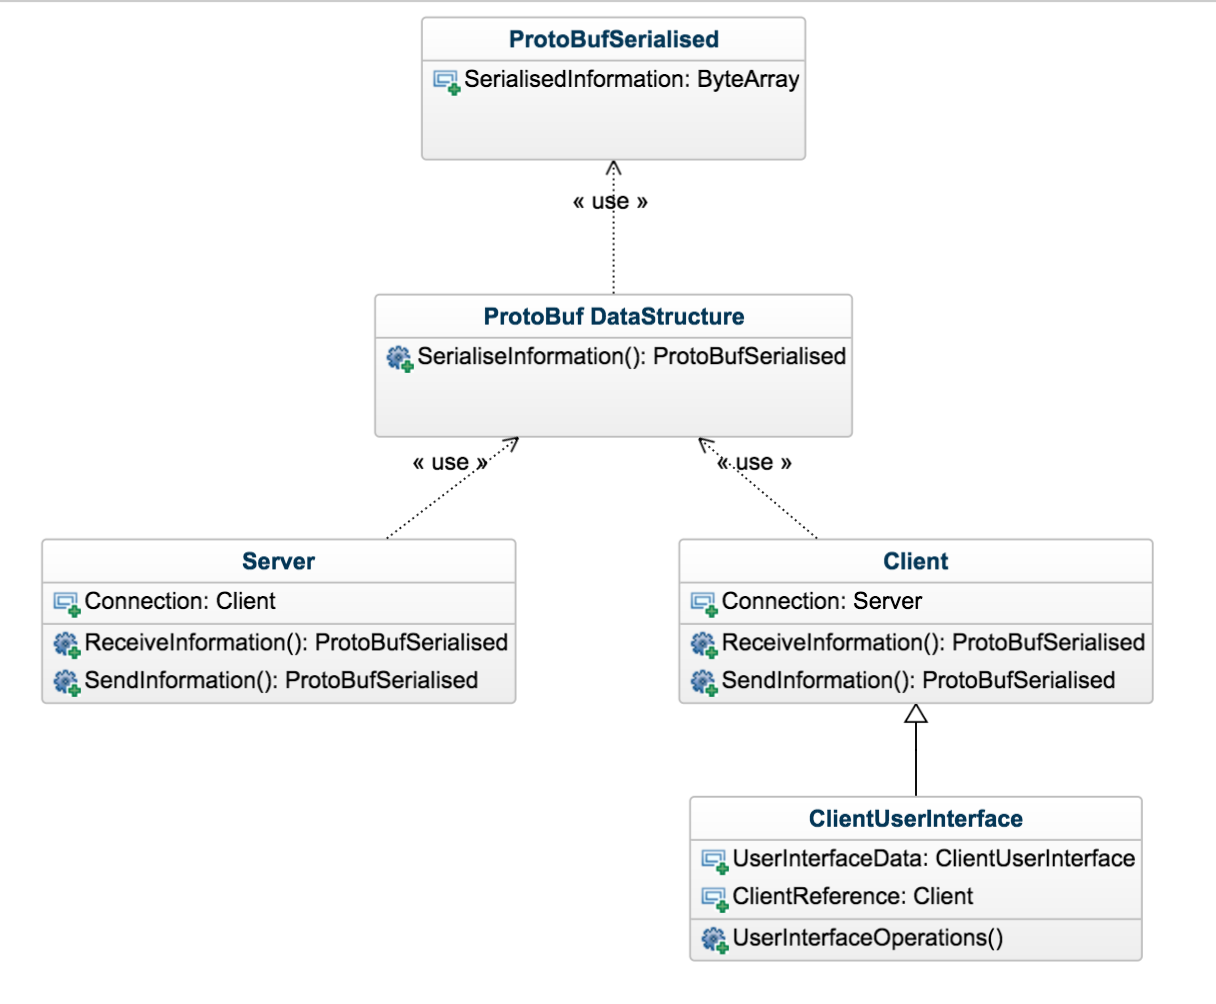
\includegraphics[width=\textwidth]{classdiagram.png}
JominiEngine and its clients have been in continuous development since the project was started, there were more features added on by the students and staff that work on it every year, due to their efforts I was not starting from a complete scratch and had a codebase with which to work with in order to produce my implementation. David Bond originally created a single player game with which the work of Helen Rankin\cite{helenrankin} added a networked element, Helen Rankin made a lot of design decisions during the implementation such as designing the protocols with which communication with the server is performed or choosing the libraries with which packets are serialised. Helen also left a barebones communication interface, this allows for Protobuf data structures to be sent and received from the server over the Lidgren UDP protocol. The above class diagram describes the overall structure of the project, during the development of a client, depending on the platform, I was tasked with implementing everything but the server. The user interface, whether it be textual or graphical, drives the client, providing the information with which to fill a request with, the request's representation before it is sent to the server takes the form of a protobuf data structure, which using the methods built into the Protobuf framework, serialises this information for transmission to the server. The server receives the information and de-serialises the information from a byte array back into a Protobuf data structure, using the values in the data structure to make the changes to the game state required.
\subsection{Text Client}
The first client I chose to implement was the command line text client; I chose this first for a few reasons. Firstly, after its completion it would provide a point from which to test the facilities of the server were working correctly, if unexpected results were obtained from running operations from the text client the code of the server relating to the operation that was being performed could be checked to ensure it was working as laid out in David Bond’s thesis. Secondly, the command line client is the least computationally demanding of the three to run, this means that in a demonstrations environment this client can be run multiple times on the same machine in virtual machines to test the limits of the amount of connections to a single server at once. Thirdly, the command line client is a C\# based client, this means that the operations codebase, the actions performed after a user has given an action to perform via the command line interface can be converted into a Class Library, then compiled into a DLL file for use in different clients written for the same platform, an example of this is the unity client provided in this project. 
\subsubsection{Build Pipeline}
To produce a working client a build pipeline had to be prepared, this involved the creation of a shell script which ran through the build process that was required depending on the system if it was currently running on. If this is a Windows system the ‘msbuild’ command must be called on the required .csproj files, if it is a Unix based system such as Linux or OSX it is required to run the ‘xbuild’ command, this is the Mono version of msbuild and it takes the same arguments. Both Linux and Windows compile to executable files which can be run as would a standard executable from command line, the path to the file is passed such as ‘./path/to/executable.exe’, however Mono on OSX requires the file path to the executable to passed to it via the mono command, to run the same file the command ‘mono /path/to/executable.exe’. To produce a shell script which could be run on any platform by a user of any skill I produced a build script, this compiles the latest version of the codebase and then runs both the server and the client with the correct commands depending on what operating system the user is running.
\subsubsection{Modifications to Server Code}
The server code I inherited had some compatibility issues when running on systems other than Windows, mostly relating to file path errors. An external Windows server is probably the best choice throughout the testing process but during the development process I did not have access to a machine running the correct configuration and I wanted to be able to attach a debugger to the server to see the information it was returning depending on the messages the client sent to it no matter which system I was running on, to achieve this I had to make some changes to the server code. This required to make different decisions based on which file paths were used when accessing log files and security keys based on the type of system that it is being run on.
\subsubsection{Structure of Program}
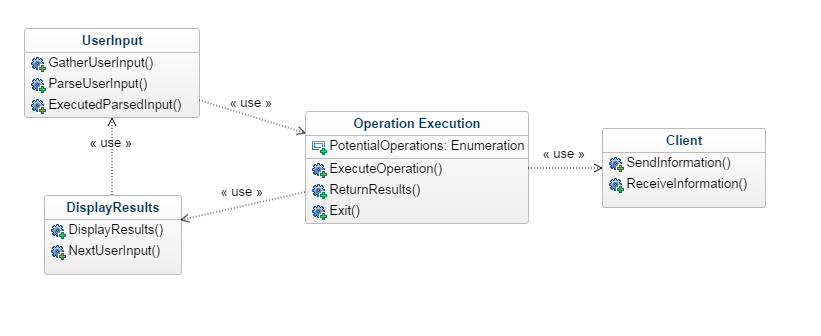
\includegraphics[width=\textwidth]{textclient.png}\\
 The text client works in a loop, it takes user input, processes it and then based on the input it receives it executes a function. The execution of the function makes use of the communication layer, this contacts the server with the user supplied information and then awaits a reply, when the server replies it then hands the information to the display class which in turn sets the client up for the next input from the user, this continues until the program is shut down or the user types the exit command.
\subsubsection{User Input Processing}
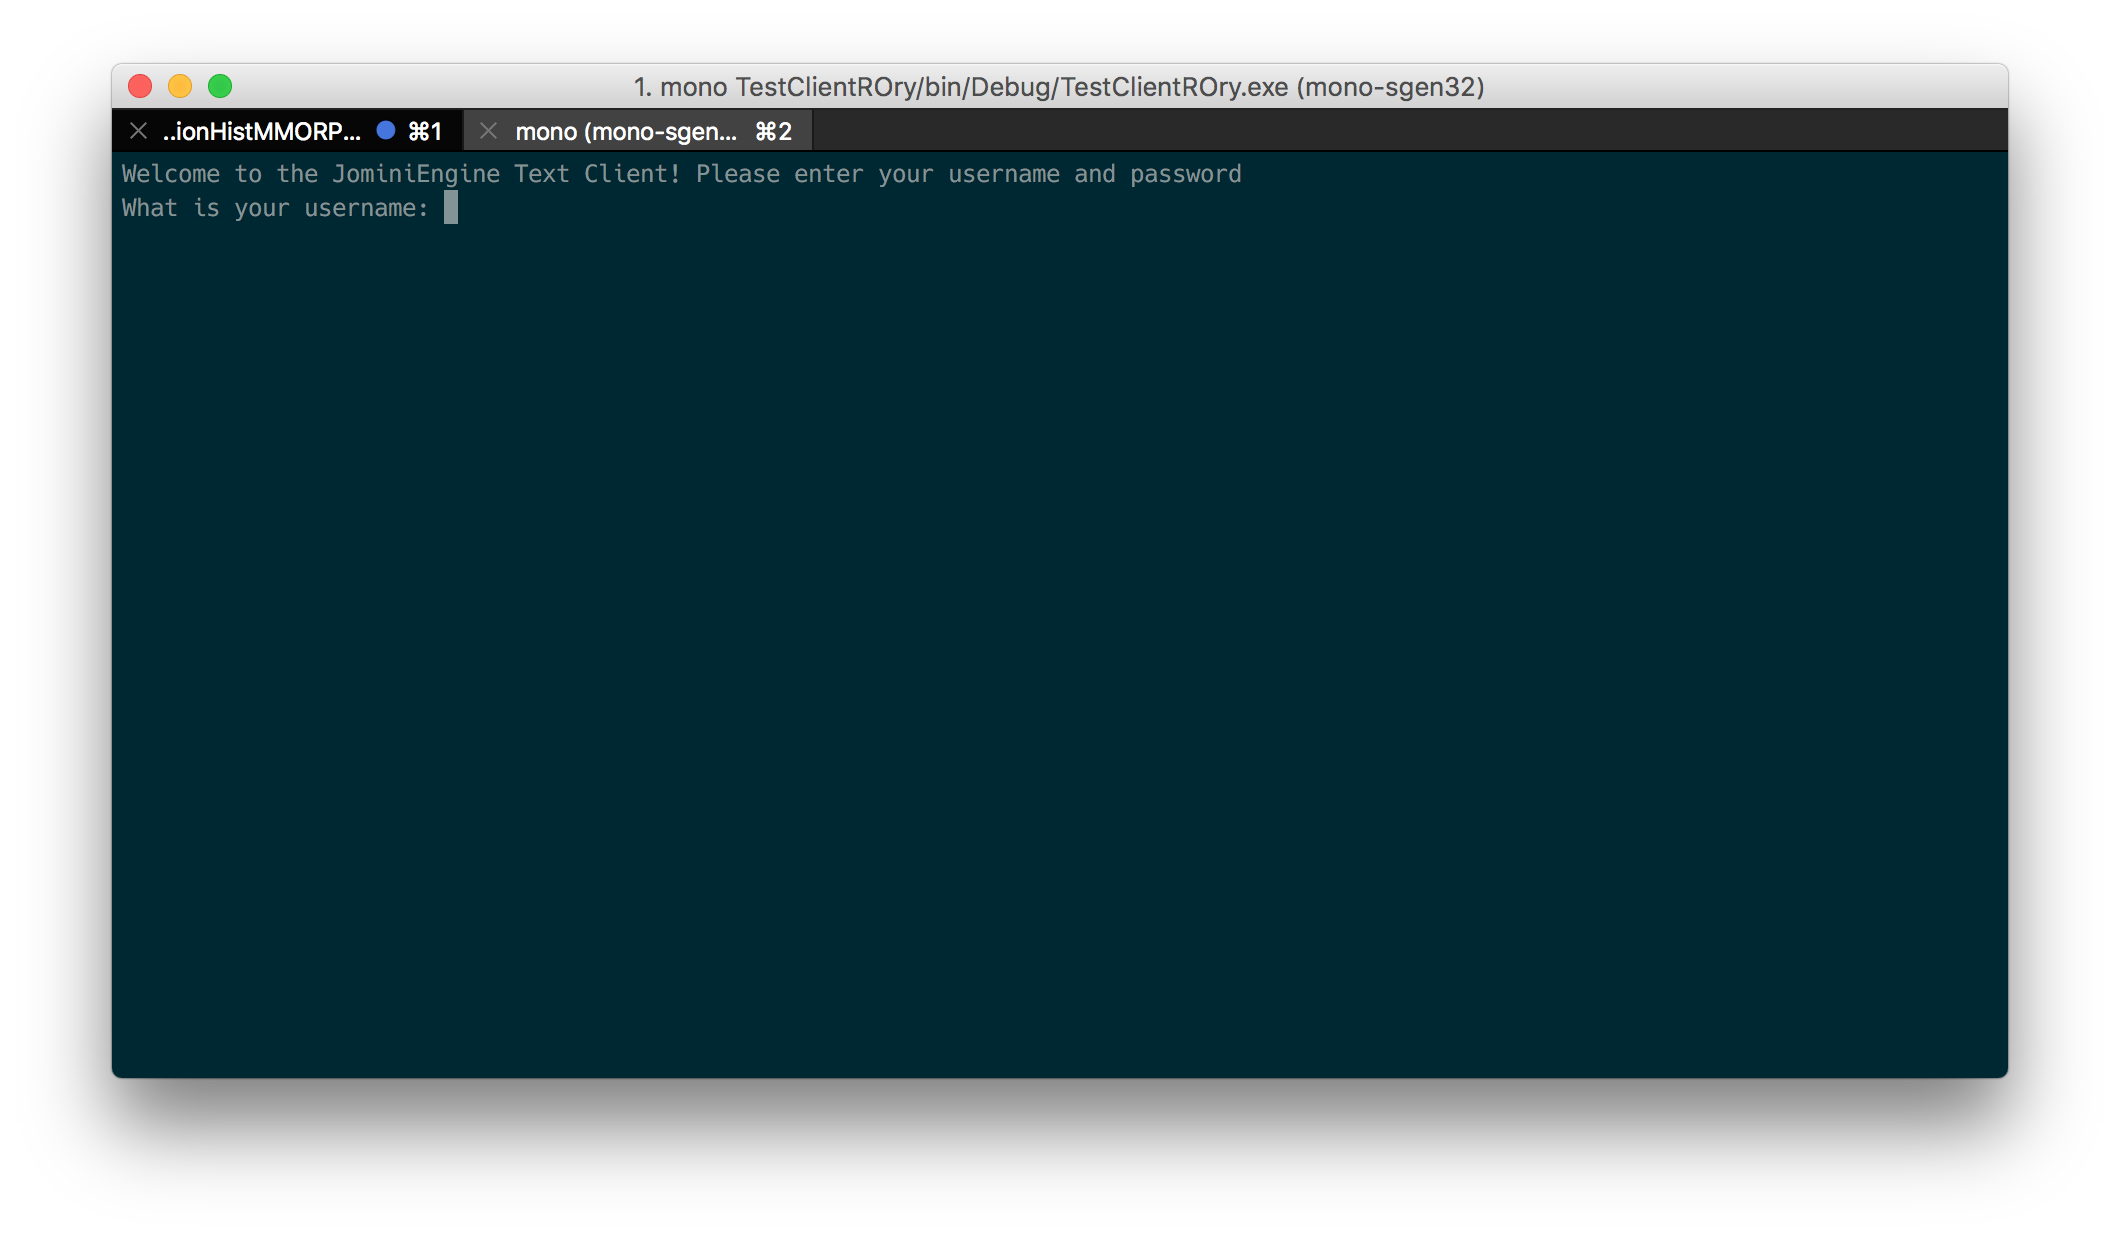
\includegraphics[width=\textwidth]{text1.png}
The structure of the command line client is split into three main sectors, there is first the part which takes user input in and processes it so it can be recognised as discernible commands with arguments if are needed. This takes place in the WordRecogniser object, which converts command line input into a UserOperation enum value, every command has a value in this enumerated type which corresponds to it. WordRecogniser is also used when a command requires a directional argument such as the Move command, this converts a direction, for example “NorthEast” into the corresponding direction in a format the program can understand.
\subsubsection{Operation Execution}
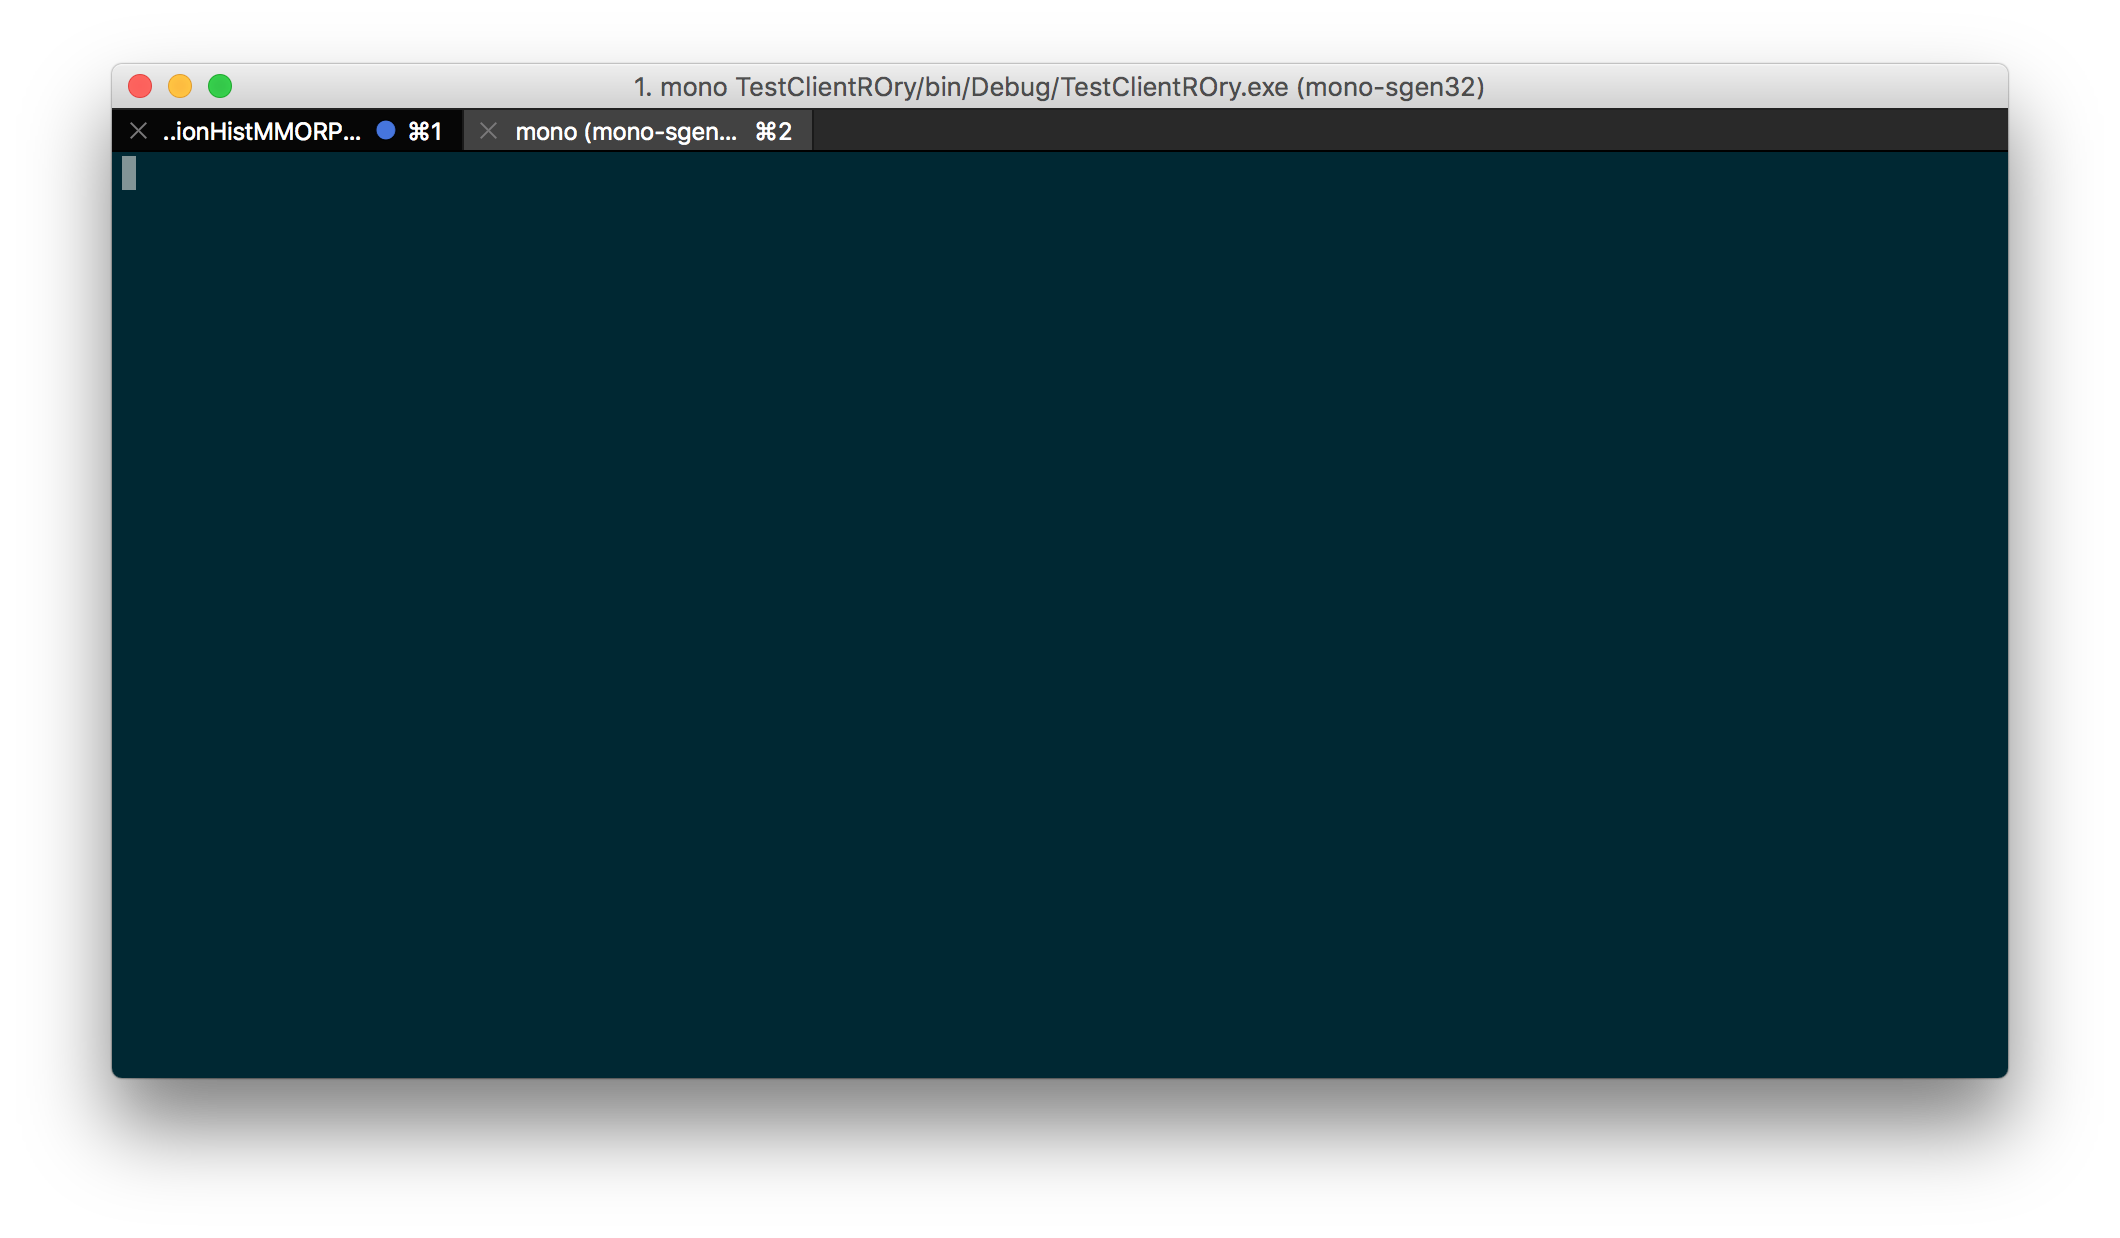
\includegraphics[width=\textwidth]{text2.png}
After the processing of the input occurs this is handled off to the required process in the PlayerOperations object, this object is the object which is abstracted out at a later point into a class library for use in other clients in the future, the program specifies which method it wishes to call and the PlayerOperations object sends the request to the server and returns the reply in a readable format. For example, if the player wished to check the contents of the current fief they would type the command “fief”, this would then be processed by the WordRecogniser object and that would specify a fief operation needed to be performed; PlayerOperations.Fief() would then be the method executed by the program which would return all the information corresponding to the desired fief as outlined in the ProtoFief object from which I inherited from Helen Rankin’s work on the expansion of SessionTypes into the Jomini engine.
\subsubsection{Displaying Data}
There is then a third and final sector of the command line client which deals with the displaying of data once it has been retrieved; when the client is notified of a reply from the server the result of that reply is handed off to the DisplayResult object, this takes in as an argument the ProtoMessage subclass relating to the command that has been performed and each command has a separate method for displaying the information retrieved from the server in the correct format.\\
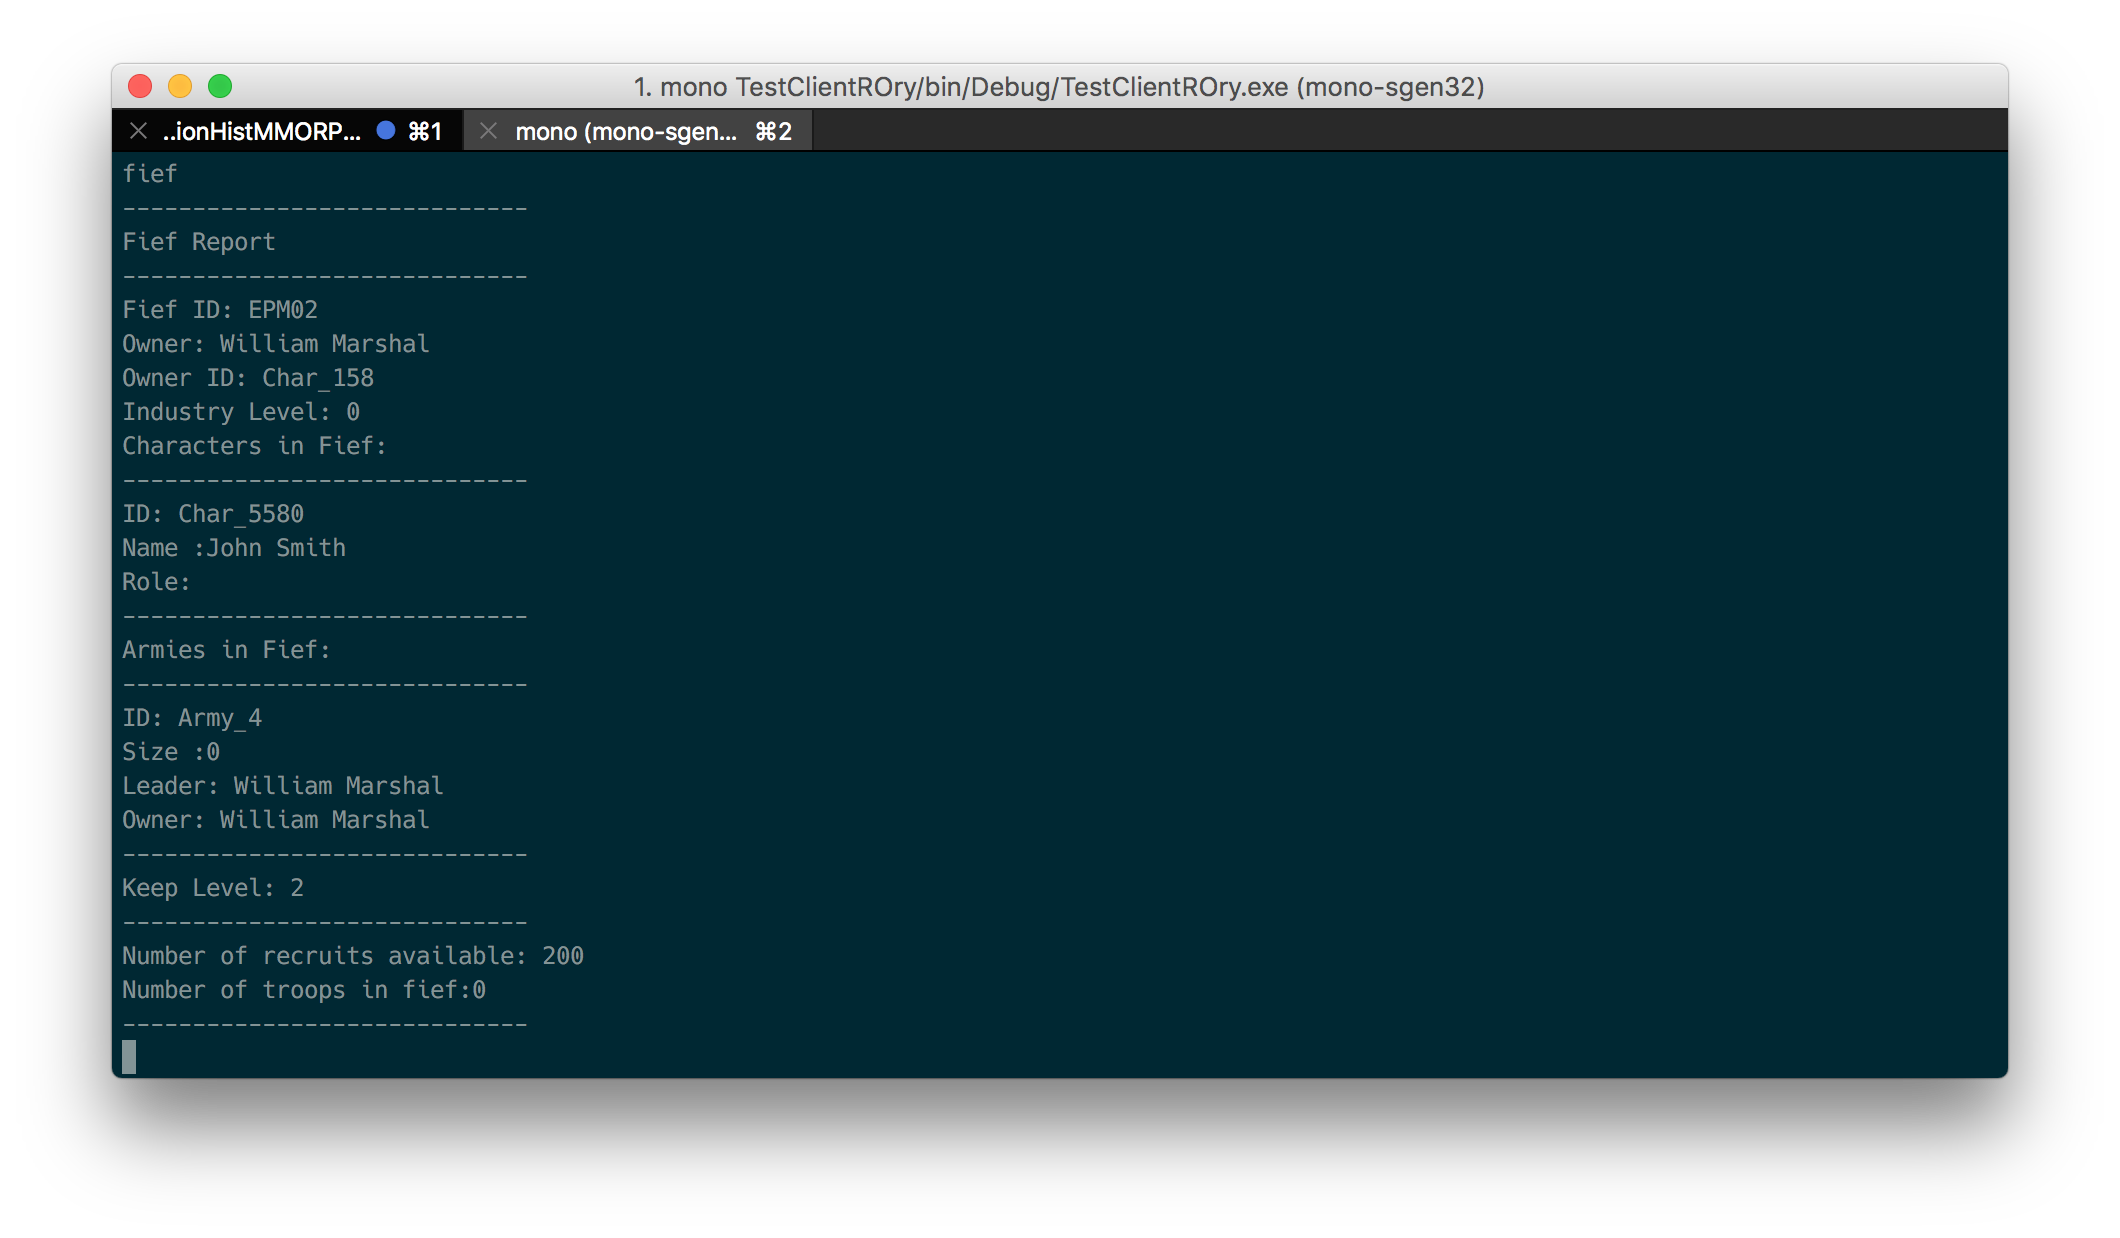
\includegraphics[width=\textwidth]{text3.png}
Above shows the report that a user is provided with if they wish to see information about the fief they are currently in, the report displays a variety of information including the armies currently within that fief, the number of troops available to recruit and the current characters found within that fief.\\
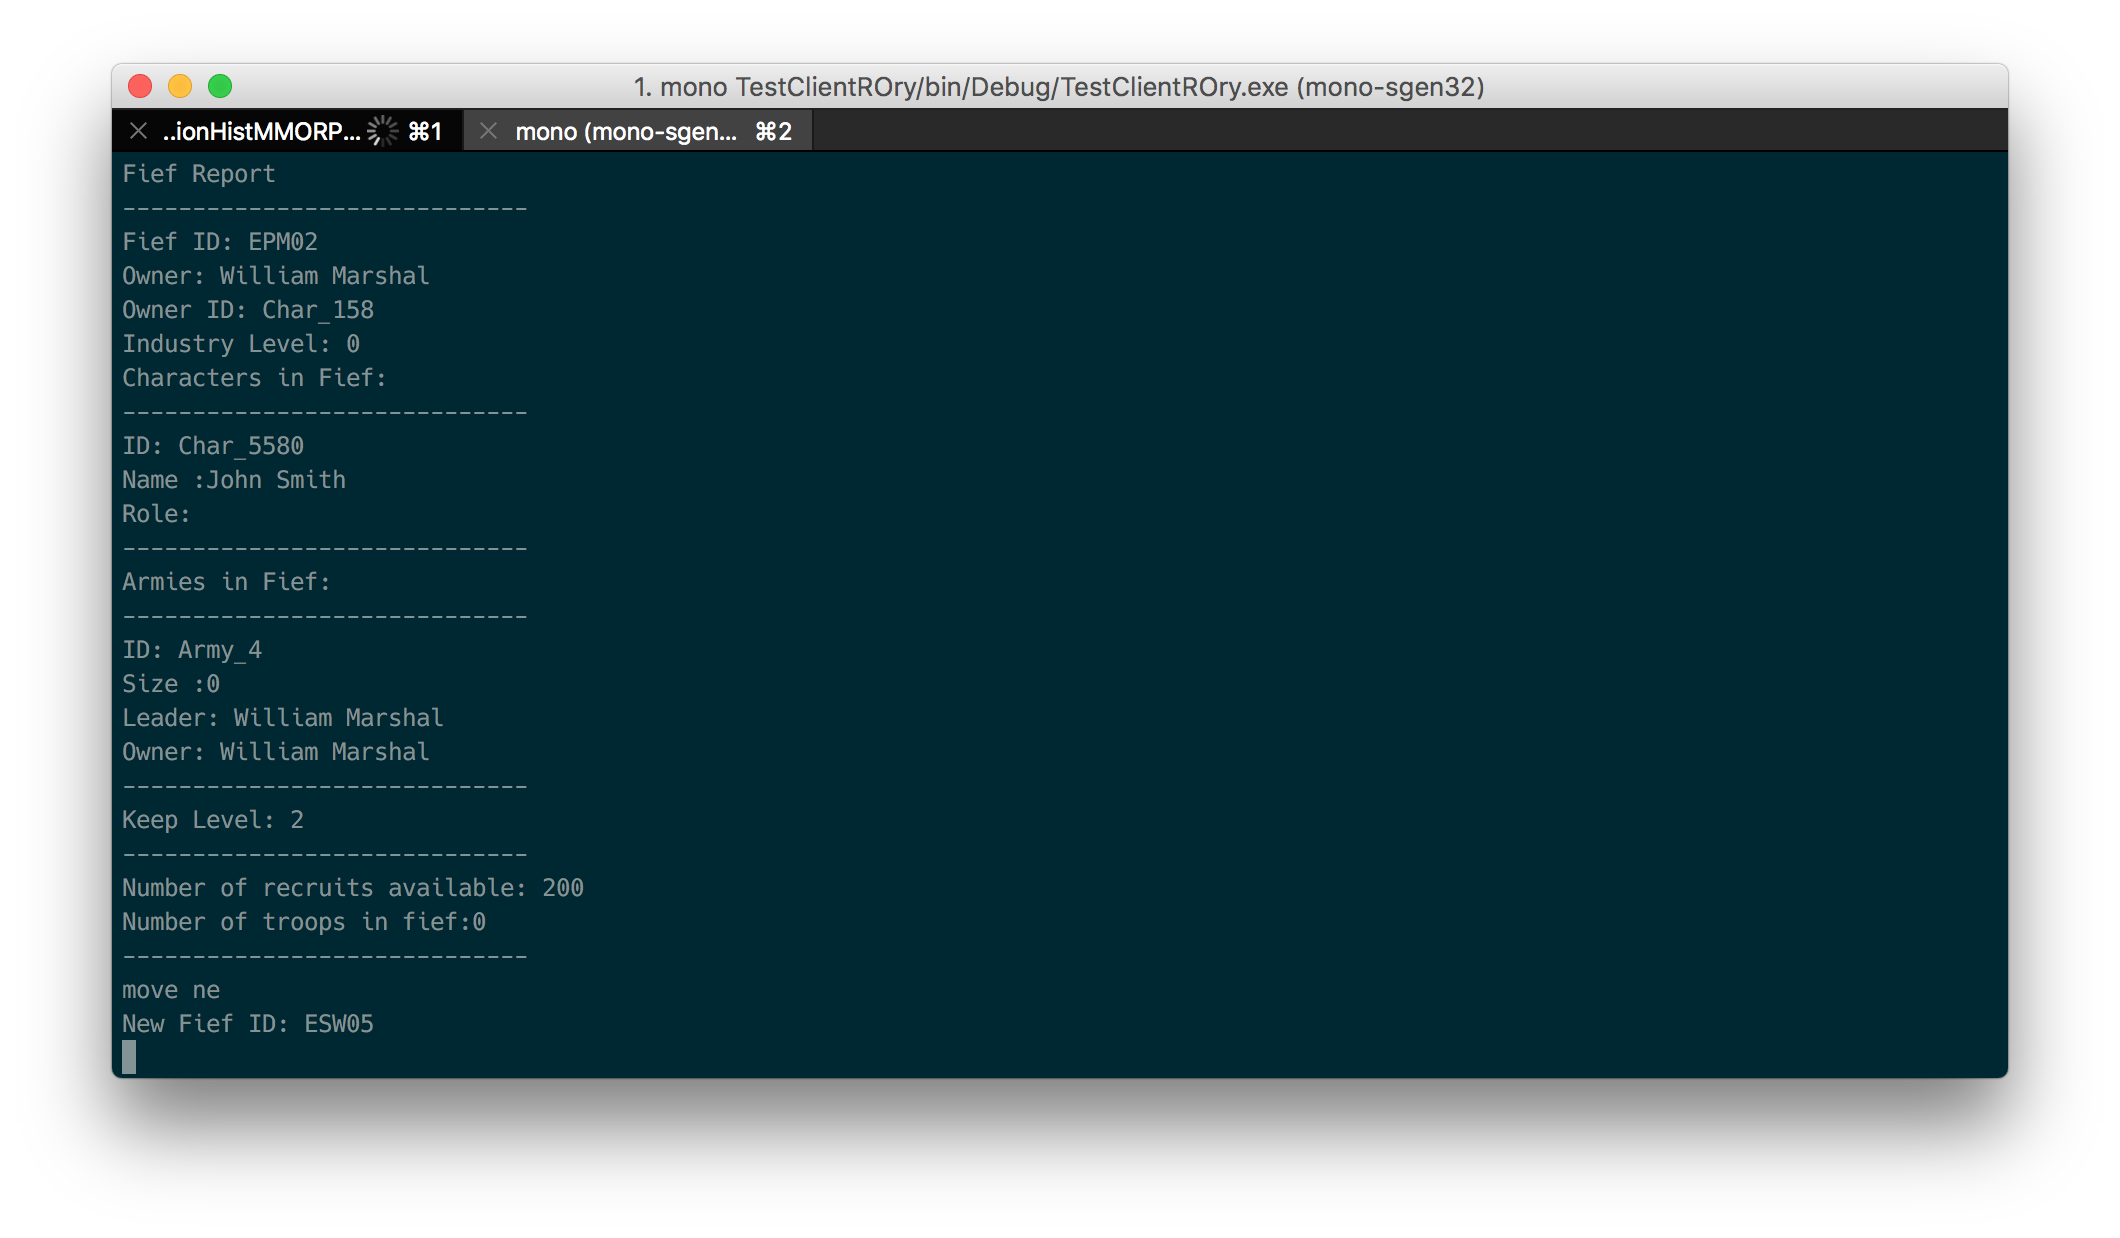
\includegraphics[width=\textwidth]{text4.png}
Above is the output of a move command, a user provides the client with a 'move' command and then supplies as an argument a direction in which to move, this can either be, for example a long hand 'northeast' or a shorter 'ne'. \\
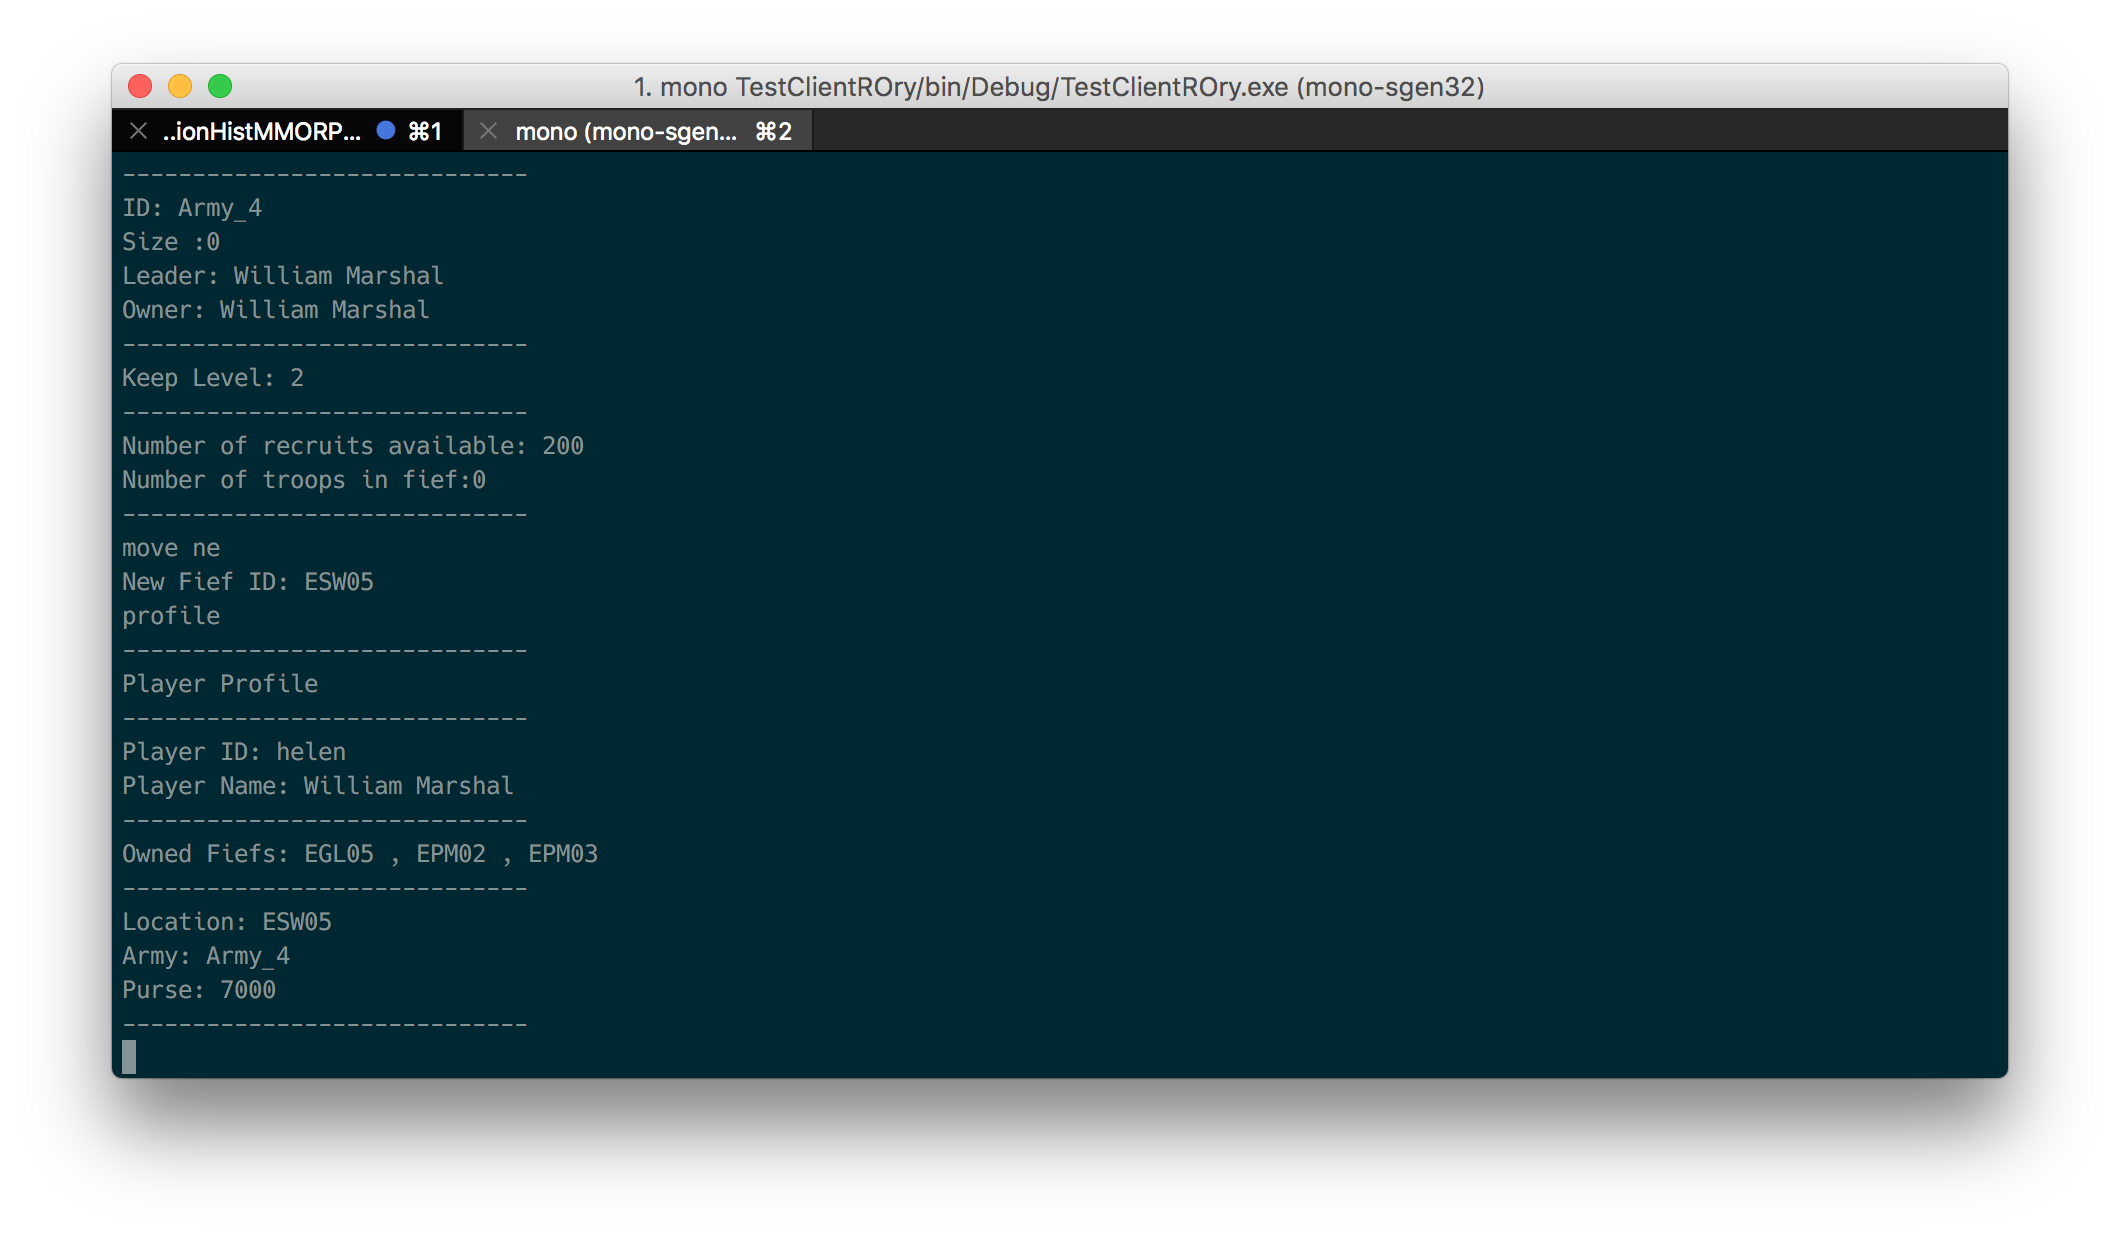
\includegraphics[width=\textwidth]{text5.png}
Thirdly we have an example of the player profile, this returns all information relating to the player's current status, including the fiefs they own, information about their army, and the amount they currently have in their purse.
\subsubsection{Dynamic-link Library}
A Dynamic-link library is a shared library which allow for programs to take advantage of the resources contained within them by adding them as a project reference, this concept is useful when, for example, developing a client for a game as the communications layer can be used in multiple contexts with different interfaces driving the execution of certain methods within the DLL. A model like this is what I chose to utilise in the Unity based client, using the communications layer I had built in earlier I created the ClientDLL class library which acts as a compilable abstraction and interface for the PlayerOperations object.
\subsection{Graphical Client}
The second part of the implementation required creating a graphical user interface for the JominiEngine client, this client had to have the same compatibility as the text client, running on multiple operating systems. Operating system user interface cross compatibility is a difficult problem to solve and opting to creating such a client limits the scope of your options for frameworks significantly, I originally attempted to write a client in the Unity framework, however for reasons I shall expand upon this proved unsuitable, in the end I opted to use the Gtk framework to create a responsive graphical user interface which ran on multiple platforms.

\subsubsection{.NET Version Incompatibility}

Unity supports scripts which are written in C\#, they are added to the Unity solution as resources and then can be run when for example events trigger or conditions are met, the version of C\# Unity supports is, under the Mono cross platform compiler, 2.6.5. This versioning proves to be problematic when making use of more recent language features, such as those used in the Protobuf-net framework, when importing the DLL file which contained references to classes written with the framework I received an incorrect versioning error message. A work around for this could have been possible, I could have decompiled the Protobuf-net classes, such as ProtoMessage.cs, to the Protobuf Domain Specific Language using the same technique I later used for the development of the Android client. This made use of an experimental method in the Protobuf serializer object, toProto(), this takes in as an argument a data structure which is annotated with the Protobuf-Net syntactic sugar, then returns the equivalent in the domain specific language, with this output I could have then used the Protobuf compiler to compile the output, targeting an earlier version of the Mono framework than currently used.

\subsubsection{Inexperience with Unity}

Another problem I had with carrying on with the development of the client using the Unity framework was my general inexperience with the platform. While with time, a client that used Unity could have been produced it is much more complex than the Gtk, the tool I settled on, to get grips with and produce a prototype. As time constraints towards the end of the project closed in and the errors with Protobuf versioning compatibility started to arise and prove themselves to be a formidable tasks in itself to get to grips with and mitigate, I made the decision to use Gtk instead.

\subsubsection{Gtk Rollout}

Due to Gtk’s cross language and cross platform compatibility I already had some experience with it via building user interfaces for a Python program, this was valuable knowledge, after setting up the Gtk build pipeline and getting to grips with the differences from Python it allowed me to get up and running much faster than if I had instead used Unity. The portability of the structure of the text client made it so a lot of the communication layer was already complete, the user interface structures to drive and display this information needed to be built around it.
\subsubsection{Structure of Program}
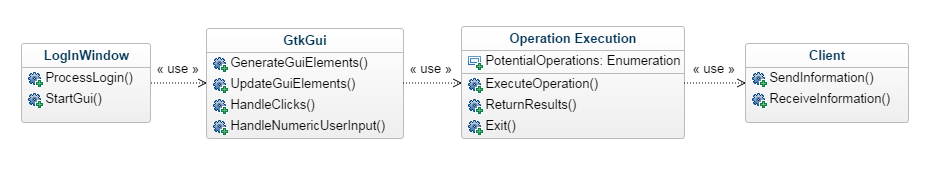
\includegraphics[width=\textwidth]{gtkclient.png}
The Gtk client has a similar program structure to the text client, however the loop that is implemented inside of the text client to capture user input is now captured within the Gtk framework. Gtk allows for the programmer to attach certain functions to event handlers, such as on a button press execute this function, this means that we match the functions for carrying out operations to the relevant button, and include the code for displaying the relevant information inside of this. On a button press, Gtk captures the event then executes the operation on the client which then waits for a response from the server and returns the result via the mechanisms described in the rest of this section.

\subsubsection{Display Grid}
Gtk offers many tools with which to build usable interfaces, however, a single window can only display one object within it at a time, therefore, we must create a grid within which to store multiple objects to display to the user, this grid is then added to the main window from where the user can interact with all the facets of the system. For our implementation of JominiEngine, 

\subsubsection{Profile and Fief Display Classes}

The information on the player, their armies, and the fiefs they visit updates frequently, a robust model, in this place an object, must be in place to display this information to the user. These classes must mirror the details within the respective protobuf datatype and have the mechanisms to take this datatype and from it construct a user interface which can be displayed. To represent the user’s profile, for example, we must look at the information stored within it, this consists of the user’s character ID, the user’s character’s name, but also contains more complex information such as an array of all the armies currently under that user’s control. The best mechanisms to display this information, native to the tools that Gtk give us, are to place them within a table grid system, therefore the display classes must take the information as input, via their constructors, and then compile them into a grid, which is then returned higher up the UI stack. Since the information in the grid is not always the same size or in the same format, for example, some users have more armies than others, we cannot keep an exact one to one reference which is easily updatable, it is impossible to keep a single label called “ArmySize” which we update the value of as the user hires more units. Therefore, whenever we wish to update the value of a the profile or the fief information display, we must destroy the old object and create it again with the new information added in via the constructor. To destroy the old information we must call the Destroy() method on the old object, this initiates a garbage collection upon the object and removes it from the user interface, this is performed from higher up the user interface hierarchy via a method, DestroyProfileTable(). After the object has been cleared redraw it by creating a new object with the information from the request to the server, this is performed on the fief display every time the user sends a move command, updating the information about the fief the user is currently in.

\subsubsection{User Interface}
As mentioned before Gtk makes use of objects named “windows” which are allowed to contain one UI element. Windows are useful when created sections of the application which are markedly different from each other, an example of this is the login screen during the setup process of our application. Before the user has logged in it is impossible to display information to them, if the UI elements were loaded before login has occurred they would contain null which is not helpful to the end user and is bad for usability. Therefore, making use of windows, we can have a login in screen which is displayed to the user when they first run the program 
\begin{center}
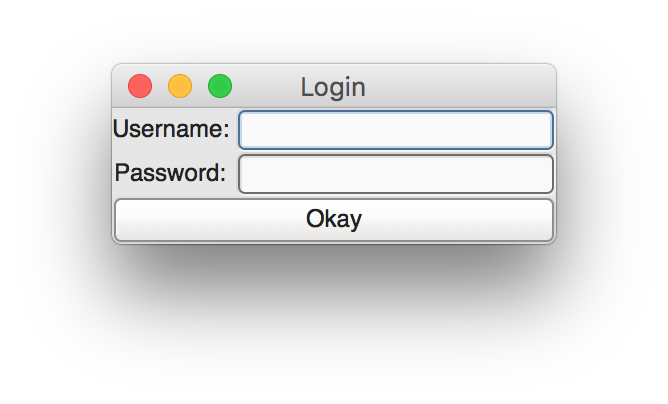
\includegraphics[scale=1]{gtk1.png}
\end{center}
This login screen prompts the user for the correct information with which to proceed, when the user has completed this task they press the ‘okay’ button to continue, there is no other possible path for them to take. When a user completes this task the login occurs and the server fetches the information which is relevant to their profile, this is then presented to the user via the display classes I described earlier.

\subsection{Android Client }

Natively Android supports the Java programming language, which it then compiles into an Android specific bytecode for execution on the Android runtime. 

\subsubsection{Android Networking}

Android applications are limited in the scope of access to the device’s hardware they are entitled to via the permissions the user allows for an application to run with. These permissions, included access to the android device’s networking stack, are compiled into an xml file in the project’s root named manifests.xml; since our application makes use of the networking stack, there is a need to inform the user of this before our application runs. Since the Android application runs inside of an emulator, the game server is hosted on a different machine to that of the client, this means that connecting to localhost where the game server is running is not possible. The Android emulator comes with a built in solution to this in the form of the reserved IP ‘10.0.2.2’, this address is an alias to the host machine’s loopback interface and allows for the emulator to access the host machine’s localhost.

\subsubsection{Protobuf-net to Proto}

Helen Rankin's server implementation made use of the Protobuf-net library for C\#, this is useful in that context as it allows for the developer to create the Protobuf message formats in native C\# with syntactic sugar added that the compiler can understand when the build process is executed, compiling native C\# objects for use on the protobuf layer. However, Java does not have a similar feature, it requires the Protobuf data structure to be written in the Protobuf domain specific language, and if it did there would need to be a re-writing of the Protobuf data types in Protobuf-net to the Java equivalent, this proved problematic, I had to try to come up with a solution which avoided this time-expensive process. I made use of the C\# Protobuf libraries Serializer.GetProto<>() method, this is an experimental method in the library which takes in a data type, in this case, the ProtoMessage superclass of all the Protobuf data structures in the C\# client implementation of JominiEngine and produces the Protobuf domain specific language implementation of the Protobuf-net C\# data structure. Once the output of this was saved to file, I could then run the result through the Protobuf compiler with a Java compilation flag to produce a Java file called HistMmorpg.java, this file contains a Java implementation of the Protobuf-net C\# data structure used in the text client ready for use on the Android platform.

\subsubsection{Networking Interface}
In order to communicate with the server I had to set re-implement the networking stack I inherited from earlier clients for sending messages between the the two. I originally began this implementation in Java, however due to some issues that I shall explain later on in the passage with regards to compatibility I chose ultimately to move the project to a Xamarin based solution for Android. The original server as created by Helen Rankin makes use of the Lidgren networking framework for C\# in order to send and receive messages on both the client and server, Lidgren formats packets in a certain way that is very specific and while some characteristics are shared with normal UDP packets they do not exactly match. There is no Lidgren implementation or Lidgren clone for Java based systems, while Java has socket utilities that provide similar tooling it is not an exact match. This proves problematic when the server is receiving packets using Lidgren’s read message utility as the current implementation does, if a client does not match the Lidgren specification it is viewed by Lidgren as an errored packet and this is rejected by the server. Java’s native implementation of the socket protocol is found in the DatagramSocket object, this is used to send DatagramPackets via the UDP protocol, it does not add any headers to the packets it sends other than the expected UDP headers for configuration purposes. Herein lies the problem with the sending and receiving of packets via Lidgren when not using the Lidgren library’s send method to package information inside a byte array before it is sent, the p00acket produced by Java’s native DatagramPacket class does not match the Lidgren specification and is rejected and marked as an errored packet even though the byte array that is sent is the same in both implementations. \\
\begin{center}
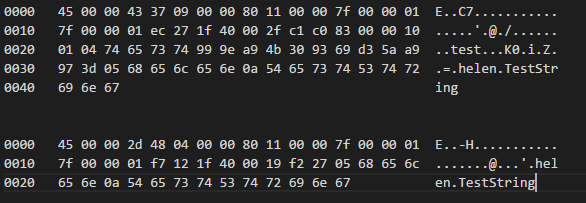
\includegraphics{packetdiff.png}
\end{center}
In the image above, the original packet sent by Lidgren is the first row of hex text, and the secondary packet send from the Java client using its socket implementation can be seen below, here the differences and similarity between the packets can be seen. Lidgren, at some point, during the sending of packets over the protocol adds extra headers, this includes information referencing the setup process of the client-side NetworkUtlityProtocol object in the client initialisation process. I attempted to discover more about the roots of this problem using the Wireshark networking monitoring utility on Windows, this proved problematic due to the fact that Windows does not allow Wireshark to monitor over the loopback address (localhost) where I run both the server and the client during the testing process. In order to mitigate the issue of not having access to the loopback address I made use of the RawCap command line utility which has the ability to monitor the loopback address for protocol traffic and then generates a .pcap file which can then can be loaded into Wireshark for deeper inspection, here the differences between the packets were laid clear and I realised the scale of the incompatibility issues for the first time. While I attempted some mitigation of this problem from the java side, including creating methods which formatted a potential Byte array that was sent from Java to include the extra headers for the Lidgren protocol, therefore allowing the server to read the packets this effort proved fruitless, I could find little documentation for Lidgren which allowed me to grasp the differences in formatting.
\subsubsection{Move to Xamarin}
The Xamarin framework allows for C\# code to be run on the Android platform under a version of Mono called ‘Mono for Android’. Xamarin also allows for apps to be compiled for the iOS platform with the same codebase, this proves to be very useful when writing cross platform mobile applications. The advantage of using Xamarin in this case was due to the networking issues I was having with implementing a client that could communicate with the server using the Lidgren framework and Xamarin would allow Lidgren in its native C\# form to be used on the Android platform. Mono for Android, however, does not implement the full C\# stack, there are some modifications to the native libraries that are included, for example, the class serialisation utilities are not implemented in the same form that they are in the standard .NET library and the console utilities are left out entirely. This proved to be problematic, the codebase used for communication with the server makes use of a large amount of features and classes which are not available in Mono for Android, more so, in order to import classes into a Xamarin application a special type of DLL, a Portable Class Library, is needed to do so.
\subsubsection{Portable Class Library}
The earlier DLL (mentioned in section 3.3.8) did not match the specification required for a Portable Class Library, and therefore I needed to construct one from scratch. Portable Class Libraries were added to the .NET platform in 2011 and aim to break away from the restrictions that come with individually compiling DLLs for each individual platform that the program could potentially be run on, when a Portable Class Library is originally created the creator has the choice to mark which platforms it will be running on and the Portable Class Library then enforces the limitations applied to C\# code for all of these platforms to the codebase. In order to create a Portable Class Library which matched the requirements I needed, a reference to the ProtoBuf data structures created for the server and client to share and communicate with, I had to bring the code from the server and client test harness created by Helen Rankin across. This proved to be an issue, the classes used as part of the Protobuf library are written using the Protobuf-net library which makes use of serialisation features not available in Mono for Android. To alleviate this issue I made use of the Shim library, this makes dummy data structures for use in place of classes used in legacy .NET code which does not comply with the limitations of a Portable Class Library, with the inclusion of this library references to all missing .NET features used were added which made the code compilable. The problem with the original JominiEngine codebase is that it is rather tightly coupled; at the heart of it it is a test harness which runs through a method starting a client and a server, leading them through a series of tests of which the outcomes are confirmed and then the codebase exits, the server and client do not operate independently of each other. Furthermore, the server and the client in parts share a codebase, they both make references to Protobuf classes which are in the same solution, they do not import the data structures from a separate solution via a DLL. This is problematic, since the Portable Class Library cannot reference these data structures exactly and has its own versions of the Protobuf data structures which mirror those of the original server and client, functionally and structurally, but with a different signature there is not an exact reference. When calling ProtoBuf methods upon the received packets from the Android client to deserialize them from their transmission state an error occurs due to the fact the data structure that is serialised, although functionally the same, is the Portable Class Library version; the only way to deal with this problem is to reimplement the entire server and other clients using the version of the data structures used inside the Portable Class Library.
\subsubsection{Structure of Program}
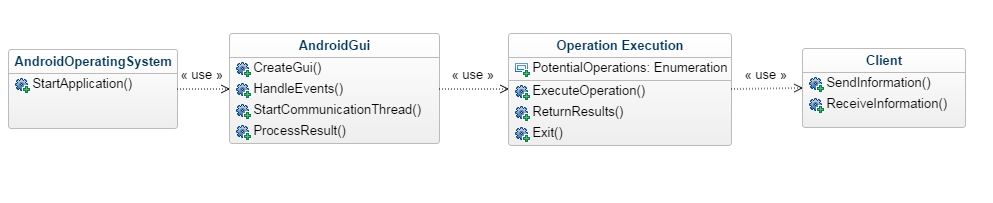
\includegraphics[width=\textwidth]{android.png}
The structure of program that the Android environment allows for is markedly different to the clients before it, largely in the way in which it forces the developer to make use of threading. Networking, which the client makes heavy use of in order to communicate with the server, is completely forbidden by the system from the main thread on which all UI operations are performed in order to reduce the chances of lag occurring. This means that when a button is pressed on an Android user interface, a new delegate is spawned on a new thread from which a response, when it is accessed is returned to the user interface.
\subsubsection{User Interface}
\begin{center}
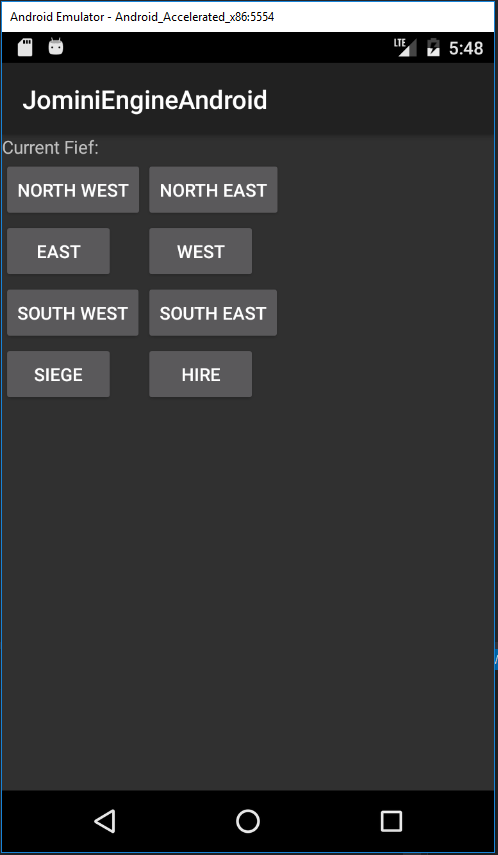
\includegraphics[scale=0.5]{jominiengine.png}\\
\end{center}
The Android user interface replicates a similar one to those that have gone before it, this helps with acclimatising the user to the program. They are presented with movement buttons, laid out in the direction with which the character would move through the map and then further option buttons with which to manipulate the status of their army or fiefs. When they select an option which requires user input, such as hiring a certain number of troops, they are presented with an input box into which the correct amount of troops to hire or other relevant action are entered.

\section{Evaluation}
\subsection{Methodology}
The methodology for the investigation into the success of the implementations of each of the clients comes from their technical proficiency. This includes the static analysis of the program which involves monitoring the quality of the codebase as is, without execution and dynamic analysis which requires the program to be executed and the quality of the end result assessed via metrics retrieved from a debugger attached. The methods I chose to use for the static analysis of the completion of the codebase are built into Microsoft's Visual Studio application, they allow for the user to run a process which generates a 'Code Metrics' table with information regarding the Maintainability Index, the Cyclomatic Complexity, the depth on inheritance and the degree to which the classes are coupled together. The Maintainability Index is a number from 0 to 100, a higher number means that the codebase is deemed by Visual Studio's analysis tool to be 'more maintainable', the Cycolmatic Complexity explores all possible code paths for the flow of the program, more complex programs with a larger logic component will have a higher value. The depth of inheritance is a reference to how many levels of inheritance the codebase has within it, if a there are large numbers of parent classes this will be a higher number, and the class coupling suggests the degree to which the classes are dependent on each other, more coupled code is more difficult to change at a later stage. Due to the nature of the ever evolving development of JominiEngine it is important that the project has maintainable, extendible clients and it is important that static analysis is performed in order to understand the current state of their implementations with regards to potential extension. Dynamic Analysis provides a window into how the program performs while it is running, this is performed by attaching a debugger to the process and observing how the program effects the computer's resources; this could, for example, include the monitoring of the programs memory footprint, or it could look at how many clock cycles an operation takes, the criteria of this is different for every client, the text client must not be demanding on resources to allow more than one instance to be run at the same time, and the Android client must not be memory intensive on a device which does not have access to as much RAM as a desktop machine. The solution for the execution of dynamic analysis finally settled upon is a tool named the 'Windows Performance Analyser', this is a tool that was created for Windows 8 which allows for the user to record the operations carried out on a machine over a certain time period and generate a log file. This log file contains information with regards to various sections of the systems resource, what API's have been called by programs, how much processing power program's made use of and the memory usage of each thread and process. From this tool, graphs can be exported and measured against each other, the results will show how much more of a demand the individual clients place on a system. It is only through the dynamic analysis process we can gain insight into the platform-suitability of each of the clients, and in turn, if they have completed their goals.
\subsection{Text Client}
\subsubsection{Static Analysis}
Using the analysis utilities built into Visual Studio on the text client project we can generate a set of results that provide us with information about the quality and extensibility of the code base. The text client has the simplest grounding of all the implementations, the overarching functions that it relies upon are relatively simple and do not require extensive library support or the usage of complex language constructs. The client is modular, with each section of the pipeline separate from the other, meaning that the code can be re-used in future projects, this should mean that the code is maintainable and avoid tight coupling. The problem area of the codebase is the display mechanisms, this requires the importing of data structures and console tooling that is not required elsewhere in the solution, it remains more tightly coupled than the other sections of the codebase due to this reliance.
\begin{table}[H]
	\centering
	\caption{Text Client Static Analysis Results}
	\label{my-label}
	\begin{tabularx}{\textwidth}{|X|X|X|X|X|X|}
		\hline
		\textbf{Application} & \textbf{Maintainable Index} & \textbf{Cyclomatic Complexity} & \textbf{Depth of Inheritance} & \textbf{Class Coupling} & \textbf{Lines Of Code} \\ \hline
		Player Command Parser and Execution & 77 &      114     &     1      &    37       &     247      \\ \hline
		Results Display & 59 &       28    &       1    &     13      &       150    \\ \hline
	\end{tabularx}
\end{table}
Since the text client is a relatively bare-bones implementation it provides a good yardstick with which to measure the capabilities of the other clients, using the figures from the results of the analysis we can question to what degree user interface libraries add complexity to the solution, having something comparative allows for conclusions to be drawn on the trade-off of increasing the complexity of the client.
\subsubsection{Dynamic Analysis}
Dynamic analysis involves the monitoring of the program as it is being executed, with regards to the text client it aims to be a low cost client which does not require significant processing power to run. Throughout all the tests we have the constant of the server executable to compare the cost of running a certain client, the server should overall, throughout all the tests, record the same average processing power usage, we can compare the cost of running a client to the average of the server to work out which client is the most demanding. In the case of the text client the below graph shows the 'weight' of running the program, weight is the percentage of CPU time in that instance that is execute the program. In the below graph the server is the yellow line and the client the blue, we see, as the client sends a request just before 9 seconds the server receives the request and then responds, the client then displays the value in the return, causing the spike in activity.  \\
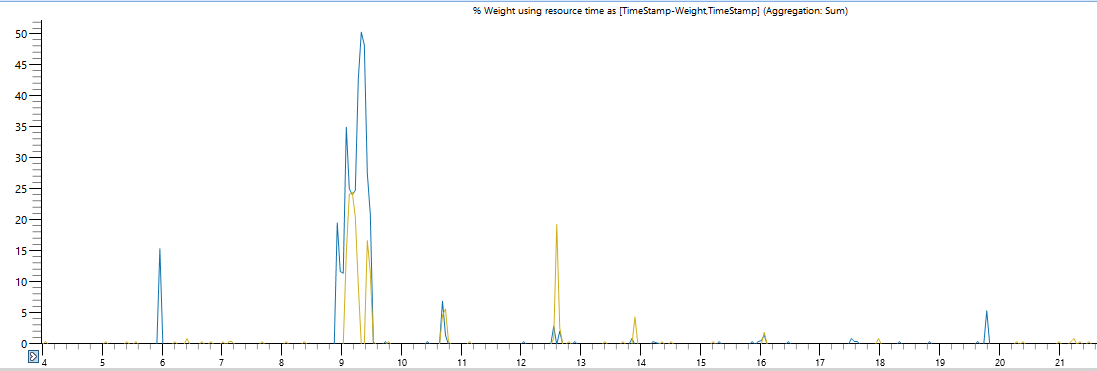
\includegraphics[width=\textwidth]{textgraph.PNG}
\subsection{Gtk Client}
\subsubsection{Static Analysis}
As we then move onto the static analysis of the Gtk client we begin to see the complexity that is derived from adding a user interface on top of the original client codebase. User interfaces framework, such as Gtk, often have a single 'User Interface' object from which all other objects such as a Button or a Label are derived from, this adds a layer of inheritance complexity from the beginning of the codebase, user interface code such as event handlers can also prove to be logically complex, this ups the clyclomatic complexity of the program. User interface components also often make use of other interface objects to build up 'windows', this can cause a class to be more tightly coupled than other, simpler solutions, all of these factors intersect with each other during the development of user interface code and this shows in the results from the analysis tool. The Gtk client is less maintainable, more logically complex, has deeper layers of inheritance and tighter coupling than the text client counterpart.
\begin{table}[H]
	\centering
	\caption{Gtk Client Static Analysis Results}
	\label{my-label}
	\begin{tabularx}{\textwidth}{|X|X|X|X|X|X|}
		\hline
		\textbf{Application} & \textbf{Maintainable Index} & \textbf{Cyclomatic Complexity} & \textbf{Depth of Inheritance} & \textbf{Class Coupling} & \textbf{Lines Of Code} \\ \hline
		GtkClient & 75 &     209      &      8     &     93      &      578     \\ \hline
	\end{tabularx}
\end{table}
\subsubsection{Dynamic Analysis}

\subsection{Android Client}
\subsubsection{Static Analysis}
The static analysis of the Android client shows similar trends to the Gtk client's results, an increase in the difficulty of maintainability, a increase in complexity, deeper inheritance and tighter coupling with regards to the results of the text client. In comparison to the Gtk client however, it is less complex and has inheritance which is not as deep, this could be do to with the optimisations of the Android operating system, code which runs on a mobile device needs to be more efficient and less bloated with regards to memory usage as it runs on a device with limited resources, the inheritance depth being shallower could be a solution to that. Gtk also has to cope with running on multiple operating systems, the expenses of achieving this could mean that code which uses the framework is more bloated than code which runs only on, for example, Android or Windows.
\begin{table}[H]
	\centering
	\caption{Android Client Static Analysis Results}
	\label{my-label}
	\begin{tabularx}{\textwidth}{|X|X|X|X|X|X|}
		\hline
		\textbf{Application} & \textbf{Maintainable Index} & \textbf{Cyclomatic Complexity} & \textbf{Depth of Inheritance} & \textbf{Class Coupling} & \textbf{Lines Of Code} \\ \hline
		Android Client & 75 &  116         &   6        &    77       &     365      \\ \hline
	\end{tabularx}
\end{table}
\subsubsection{Dynamic Analysis}
When performing Dynamic Analysis of the Android client it is important to note that it is very difficult to monitor the traffic of the Android client exactly due to the fact the code runs in an emulator. The Android emulator contains all of the processes running within the phone's operating system and conceals them from the host machine, this is problematic, as when the simulator is run it is difficult to determine if the current process is a operating system task on the simulator or a spike cause by an interaction with the client. Due to this obfuscation it is difficult to determine exactly what the cause of computational weight spikes are, however, the weight spikes in this graph are much larger than those of the text client. This could be due to the fact that there are operating systems features being run at the same time which make processing less efficient and more demanding, or it could be due to the fact the Android client is less efficient, it is hard to give a truly honest answer with the tools at hand. It is possible to use the Xamarin Profiler application in order to gain a deeper insight into the current status of a Xamarin application, however this is only possible with the premium 'Visual Studio Enterprise' version of Visual Studio, which is paywalled and not accessible with a student Visual Studio license.
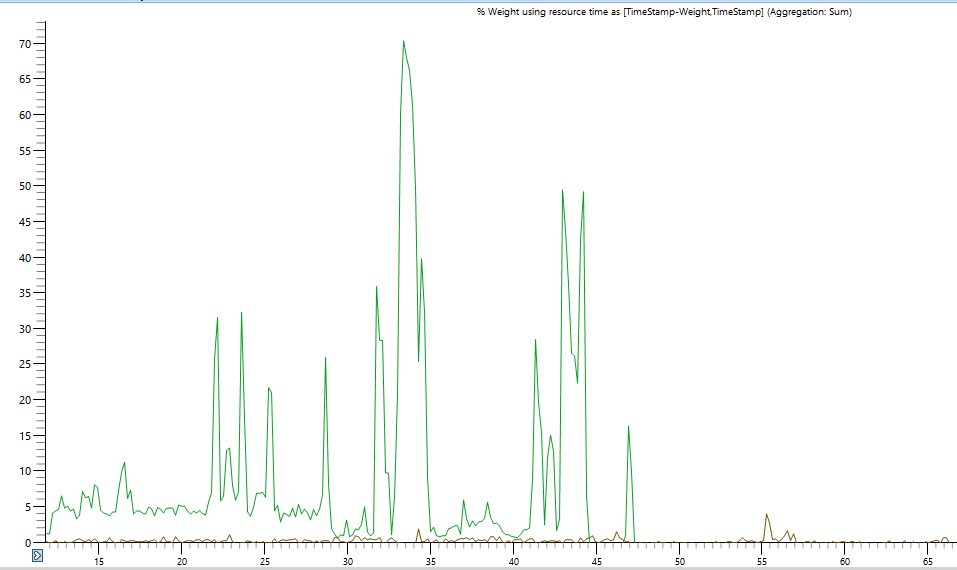
\includegraphics[width=\textwidth]{androidgraph.PNG}
\section{Conclusion}
To conclude, the completion of the clients has been taken as far as it is possible to do so without large restructuring of the server codebase. The text client and its underlying codebase provide a sound structure with which to produce more clients, written in C\#, in a similar manner in the future. The Gtk client provided an usable interface to this underlying structure, allowing for a user who does not have experience with command line tools an opportunity to use the JominiEngine in future. The Android client, for all its difficulties with implementation, showed that it would be possible to create a mobile client with restructure of the server code and the codebase of the other clients that have gone before.

Section 3.2 clearly displayed the structure to which the potential client had to fit into, through this analysis I provided a good introduction to any future developer of how the client and server communication occurs and the components which must be developed in order to make a client for JominiEngine. Section 3.3 expanded upon the process of implementing the Text client, why I chose to implement the text client first, and provided an introduction to the nuances and intricacies of the JominiEngine environment. From the implementation of the Text client a robust structure with which to build and execute clients was produced, the shell scripts I wrote allowed for anyone who wanted to test the clients to clone the repository and start the server with a single command, removing a degree of technical knowledge required to use the clients. I then went on to explain the mechanics behind the text client, showing the modularity of the program and how that lent itself to the reuse of code in future clients. I showed how I captured the input from the user and processed it into a meaningful command, after the command had been parsed I then showed how the execution of the request to the server occurred and the result displayed to the end user. Finally, in section 3.3.8, I showed how the codebase from the text client could be captured within a dynamic link library for future reuse in other codebases, simplifying the process of creating new clients from the same footprint as the command line client.

In section 3.4 I described my experiences with implementing a graphical user interface for the JominiEngine. The original implementation in Unity proved to be a problematic avenue to consider, and I showed, from the research and attempt to do so, the reasons that this solution was a sub-optimal choice for the implementation of a graphical user interface within the timeframe allowed. I then explained the reasons for finally settling with Gtk as the graphical user interface library, I show the limitations and use case for Gtk and explain how I used Gtk to create the client. The Gtk client makes use of the build pipeline and communications layer generated from the implementation of the command line client and I show how this aided me, reducing the possibility for errors and speeding up the development process.

Section 3.5 begins with a description of the Android platform and the limitations that must be worked within to create a client that works on it. I originally attempted to implement a Java client, I described my experiences with the Android networking stack and the changes that had to be made to the client to accommodate this. I then showed how a developer would take the data structures that are used in communication with the server over a Protobuf protocol and port them over to a different programming language, in this case Java. I then showed the problems with library incompatibility, I showed what the Lidgren communications library requires of packets that are sent to it and why Java was unsuitable for achieving this. I then moved to Xamarin, describing my thought process behind the move and the differences from Xamarin and native code. I showed how to take data structures from the server and implement them in Xamarin via a portable class library, and I showed the limitations that come with that when serialising information, sending it, and deserialising it on the other side of the communication. I then explained what the structure of an Android program would have to require in order to communicate with the server and the allowances the user interface must make to facilitate this.

My evaluation carried out a technical static and dynamic analysis of all three clients, showing how different clients changed the structure of the codebase and the running of the program. I showed through static analysis how adding user interface libraries or changing the platform that the program was running on affected the complexity and maintainability of the codebase, how adding a user interface framework affects the degree of inheritance complexity and the tradeoffs that occur by doing so. I then showed through dynamic analysis how the codebase informs the execution of the programs, where extra demands on resource come from and how that fits into the context of the client’s respective platforms. I then finally provided a summation and comparison of the differences in results from the static and dynamic analysis of the clients, explaining what I expected and what I received.
\subsection{Future Work}

The areas for expansion of the project mostly come from a refactoring of the server technology, to push JominiEngine onto new platforms it must abandon the tooling that has caused issues in development. The removal of Lidgren and the implementation of another communications library which fits the standardised UDP protocol would be extremely useful when exporting JominiEngine clients onto new platforms. The problems I came across in the attempted implementation of a Java based android client caused a major restructuring of the solution, however, this would not have been a necessary decision to make if the server did not use Lidgren, this would be the same for any hypothetical client written in a language other than C\#, a functional client in a language like Haskell would be impossible due to the fact there is not a Lidgren implementation it can use, this limits the availability and success of JominiEngine. 
More work is also needed to de-couple the client and server code, at the moment they are far too closely linked and it is very hard to draw a line where one ends and the other begins when looking through the codebase. The Protobuf data structures used within the server’s communications layer need to be moved to an external Portable Class Library source, they can then be imported in as a dependency, this removes any possible incompatibility issues between mobile clients and desktop clients by making them all share the same data structures for communications.
Other advancements would include the construction of new clients running on different platforms, perhaps a web application could be written which allows the user to connect from their browser. An application written using up to date JavaScript technology such as node.js could completely cut out the native code dependency entirely, all the user would need to operate JominiEngine would be a modern web browser on the device of their choosing.
	\newpage
	\section{Bibliography}
	\printbibliography
	\newpage
	\section{Appendix}
	\subsection{SUS Form}
	\centering
	\includegraphics[page=6]{sus.pdf} 
	\subsection{UML Diagram}
	\centering
	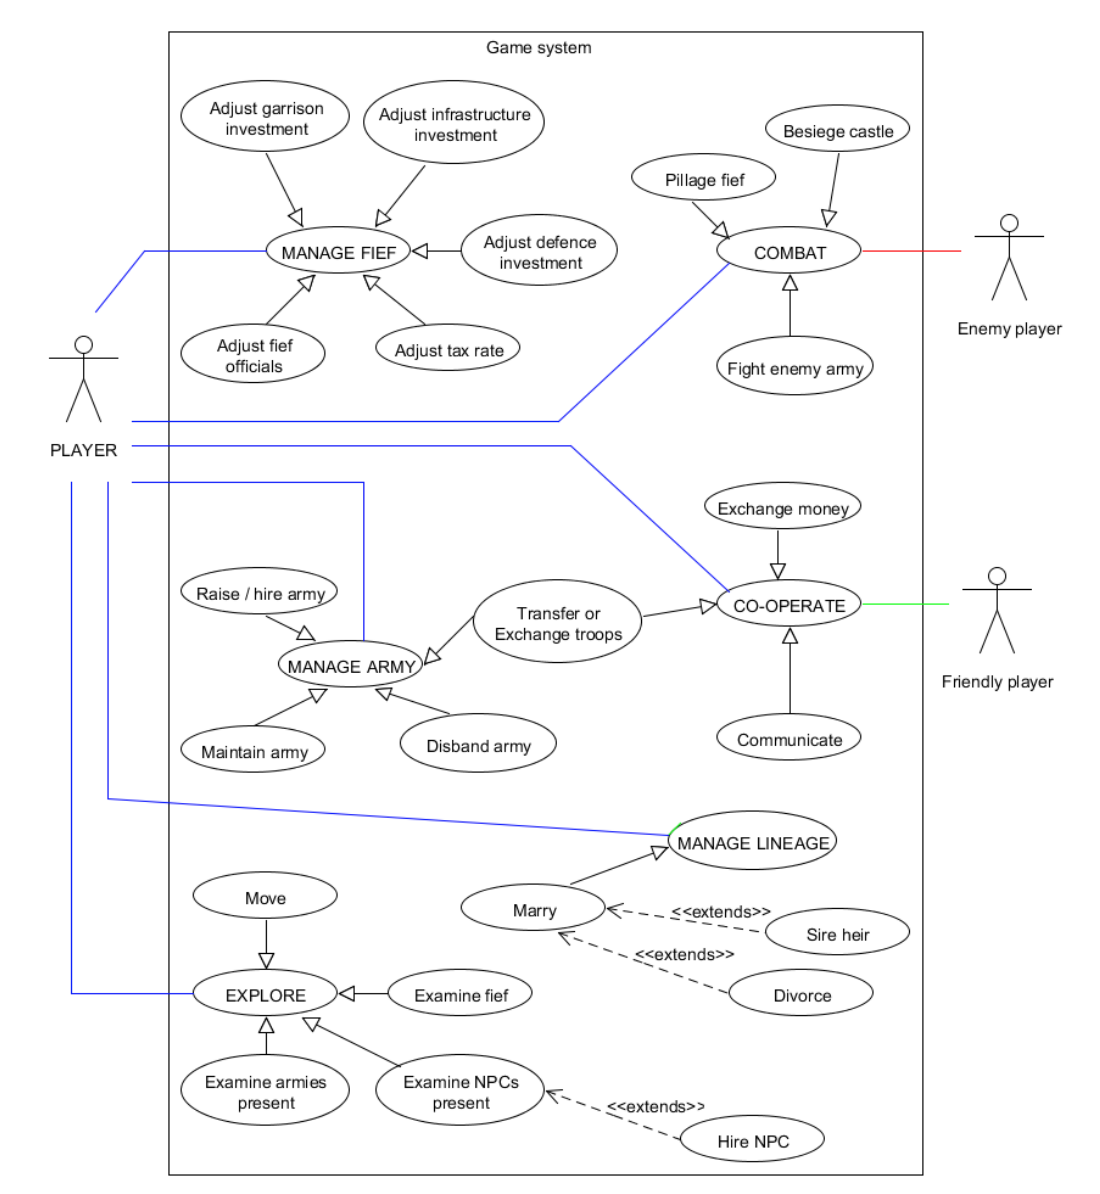
\includegraphics[width=\textwidth]{gameUML}
\end{document}
